\documentclass[a4paper,12pt,twoside]{article}
\usepackage[utf8]{inputenc}
\usepackage[british]{babel}
\usepackage[acronym]{glossaries}
\usepackage{textgreek}
\usepackage{blindtext} % jep just that
\usepackage{wrapfig} % das ist für die im Text eingebauten Figures
\usepackage[margin=1in,bindingoffset=.2in]{geometry} %titlepage
\usepackage{float} 
\usepackage{xcolor}
\usepackage{adjustbox}
\usepackage{csquotes}
\usepackage{hyperref}
\usepackage{ragged2e}
\usepackage{textcomp}
\usepackage{attachfile}
\usepackage{graphicx}
\loadglsentries{acronym.bib}
\usepackage[ddmmyyyy]{datetime} %fürs Datum in der Eigenständigkeitserklärung
\renewcommand{\dateseparator}{.} %fürs Datum in der Eigenständigkeitserklärung
\newcommand{\HRule}{\rule{\linewidth}{0.5mm}}
\newcommand{\fakesection}[1]{%
\par\refstepcounter{section}% Increase section counter
\sectionmark{#1}% Add section mark (header)
	\addcontentsline{toc}{section}{\protect\numberline{\thesection}#1}% Add section to ToC
}
\author {Florian Kühne}
\date{
	Faculty of physics, University Duisburg-Essen, Lotharstrasse 1,\\ D-47057 Duisburg, Deutschland\\
		Faculty of chemistry, University Duisburg-Essen, Universitätsstr.5,\\ D-45141 Essen, Deutschland\\
	
	\today
}
\title { Master thesis \\
Local and non-local relaxation dynamics of hot carriers by linear photoemission}

\usepackage{fancyhdr}
\pagestyle{fancy}
\setlength{\headheight}{15pt} 
\fancyhead[LE,RO]{\leftmark}
\fancyhead[RE,LO]{}
\fancyhead[CE,CO]{}

\fancyfoot[LE,RO]{\thepage}
\fancyfoot[CE,CO]{}
\fancyfoot[RE,LO]{}

\begin{document}
\begin{center}
\thispagestyle{empty}
\includegraphics[height=4cm, width=\columnwidth]{logo_en.jpg}\\[1cm] % Include a department/university logo - this will require the graphicx package

\textsc{\LARGE Master thesis}\\[0.5cm] % Name of your

\HRule \\ [0.5cm]
{{\huge \bfseries Local and non-local relaxation dynamics of hot carriers by linear photoemission}} \\ [0.2cm] % Title of your document
\HRule \\ [1cm]

	Faculty of physics,\\ University Duisburg-Essen, Lotharstrasse 1,\\ D-47057 Duisburg, Deutschland\\ [0.2cm]
Faculty of chemistry, 
\\University Duisburg-Essen, Universitätsstr.5,\\ D-45141 Essen, Deutschland\\ [0.2cm]
to obtain the degree\\ 
M. Sc.\\ 
by \\ [0.5cm]

{{Florian Kühne}}\\  [2cm]

Erstprüfer:\\
Prof.\,Dr.\,E.\,Hasselbrink\\
Zweitprüfer:\\
Prof.\,Dr.\,U.\,Bovensiepen\\[2.5cm]

Duisburg,\,Germany,\,\today\\

\end{center}

\newpage
%\newgeometry{margin=1in}
%\maketitle
%\thispagestyle{empty}
%\restoregeometry

\newpage
\null
\thispagestyle{empty}
\newpage
\pagenumbering{Roman}
    \section*{Abstract}
        \addcontentsline{toc}{section}{Abstract}
\renewcommand{\baselinestretch}{1.2}\normalsize
This thesis utilised a \textit{time resolved} linear photoemission (\textit{tr}-LPE) spectroscopy technique with a femtosecond resolution in a pump-probe scheme to analyse the transport mechanisms and relaxation of laser excited non-equilibrium electrons in a \gls{au} / \gls{fe} epitaxial heterostructure system. The motivation of the work was to observe ballistic propagation in \gls{au} / \gls{fe} layered systems. Previous efforts have shown, that the relaxation times increased with lower energies due to an decreasing phase space for electron-electron scattering. This study aims at detection of electrons and holes which have relaxed from their primary excited states to the Fermi-level during their propagation in the heterostructure, identification of their relaxation pathway and analysis of their energy content. The material system \gls{au} / \gls{fe} / MgO(001) was chosen, because of the epitaxial growth and the pristine interface conditions, as shown by Alekhin et al. \cite{Alekhin2017} and Razdolski et al. \cite{Razdolski2017}. Here \gls{au} is being probed as the propagation layer, where the transport occurs. To differentiate the separate contributions of transport and relaxation a previously developed back side pump / front side probe technique was used along with the usual front side pump / front side probe. In the back side pump / front side probe configuration \gls{fe} acts as an excited electron injector layer, because of the strong absorption. But in case of front side pump / front side probe \gls{fe} acts as a sink for the excited electrons due to the shorter mean free path in \gls{fe} than in \gls{au}. The dynamics are going to be studied by varying the thickness of the \gls{au}-layer. 
The work of Beyazit et al. employed \textit{tr}-2PPE and provides insights into the non-equilibrium dynamics, but lacked insight for electrons close to the \gls{ef}. The novelty of this work is that with \textit{tr}-LPE the region from \gls{ef} to the pump photon energy can be probed above \gls{ef}, giving complementary data to previous experiments \cite{beyazit2019}. This is as well proof of principle for the \textit{tr}-LPE setup in back side pump configuration. Besides the extensively studied excited electron states, \textit{tr}-LPE allows the observation of hole states below the Fermi-level and their relaxation back into thermal equilibrium through recombination. An effort to further consolidate the understanding of how electron and hole relaxation dynamics interact and compete with the transport effects into the heterostructure is made here. This work shows that optically excited electrons which propagate through several nm thick \gls{au} layers, relaxes towards the Fermi-level and forms a Fermi-Dirac distribution with an increased excited electron temperature of about $50\pm25\,\mathrm{K}$. Furthermore, the energy content was found to be $1.48\,\mathrm{\mu J/cm^2}$ at maximum with a pump fluence of $70\,\mathrm{\mu J/cm^2}$ and relaxes after $800\,\mathrm{fs}$ to a value of $0.08\,\mathrm{\mu J/cm^2}$ through electron-photon scattering. A delay in peak energy density $U(E,t)$ of a few ten femtoseconds and a longer relaxation was found for the back side pump experiments, where the electrons propagated through the \gls{au} layer, with repopulation through secondary electrons being a major part of the relaxation. This work could measure depleted ground states as well as excited electrons, these electron holes below the Fermi-level exhibit a similar relaxation dynamics to the excited states, decaying on a timescale of $500\,\mathrm{fs}$.
%\\
%This work shows that optically excited electrons which propagate through several 10 nm thick Au layers relax towards the Fermi and form a Fermi-Dirac distribution with an excited electron temperature of X+-Y K. Furthermore, the energy content was found to be $1.48\,\mathrm{\mu J/cm^2}$ at maximum with a pump fluence of $100\,\mathrm{\mu J/cm^2}$ and relaxes with x ps by e-ph scattering to a temperature of ...
%\\
%By analysis of the LPE signal as a function of pump-probe time delay an energy dependence for the peak intensity delay, like in Beyazit et al. \cite{beyazit2019}, could be shown. In case of back side pump the analysis of electrons showed the same behaviour with lower energy electrons arriving later at the detector than the electrons with higher energy. This effect is thickness dependent indicating transport processes. Because the 'hot' electron dynamics around the Fermi-level are measured secondary electron dynamics are observed repopulating lower excited states and competing with the relaxation dynamic. Front side pump showed no delay in peak intensity, because the electrons did not have to propagate through the \gls{au}-layer. Laser calculations done in this work, show that for back side pump the excitation is predominantly in \gls{fe} with negligible excitation in \gls{au}, while in front side pump the \gls{au}-layer is homogeneously excited creating a gradient free non-equilibrium electron distribution. By determining the energy density it was demonstrated that in back side pump more energy density reaches the \gls{au} surface with thinner \gls{au} layers, dissipating less incident energy during propagation, while in front side pump the energy density decreases with decreasing film thickness. Combination of the calculated incident laser absorption with the measured energy densities after propagation show, that in front side pump a bigger proportion of the actually absorbed energy reaches the detector compared to back side pump. For back side pump the efficiency of injection decreases with increasing film thickness. This loss of energy density is attributed to scattering events during propagation through the \gls{au}-layer.  Through careful analysis of the energy resolved transients a spectral feature close to the Fermi-level,exclusive to back pump, could be identified. This peak is ascribed to d-band electrons in \gls{fe}. 
\\
%\begin{itemize}
  %  \item "femtosecond" time resolved linear photoemission 
 %   \item epitaxial Fe/Au/MgO(001) material system
 %   \item laser excited nonequilibrium electrons/holes 
 %   \item mention explicitly tr-2PPE. With this you can link to tr-ARPES and why you want to do it
%\end{itemize}


\renewcommand{\baselinestretch}{1.0}\normalsize
\newpage
%\null
%\thispagestyle{empty}
%\newpage
\LARGE
Lokale und nicht lokale Relaxationsdynamiken von angeregten Elektronen und Löchern analysiert durch zeitaufgelöste lineare Photoemission
    \section*{Zusammenfassung}
        \label{Zchap}
\addcontentsline{toc}{section}{Zusammenfassung}
\renewcommand{\baselinestretch}{1.2}\normalsize
In dieser Arbeit wird das zeitaufgelöste lineare Photoemissionsmessverfahren (\textit{tr}-LPE) mit einer femtosekunden Auflösung in einem Pump/\,Probe-Schema verwendet um die Transportmechanismen von Laser angeregten nicht-gleichgewichts Elektronen in einem Au / Fe epitaktischen Heterosystem zu analysieren. Die Motivation dieser Arbeit war die Beobachtung von ballistischer Propagation in \gls{au}\,/\,\gls{fe} Schichtsystemen. Bisherige Arbeiten haben gezeigt, dass die Relaxationszeiten bei geringeren Energien ansteigen, wegen des sinkenden Phasenraums für Elektron-Elektron Streuung. Das Ziel dieser Studie ist die Detektion von Elektronen und Löchern, welche von ihrem primären angeregten Zustand während der Propagation im heterogenen Schichtsystem zum Fermi-Niveau relaxieren, ihre Relaxationswege zu identifizieren und die Analyse ihres Energiegehaltes. Das Materialsystem Au / Fe / MgO(001) wurde ausgesucht, wegen dem epitaktischen Wachstum und makellosen Grenzflächen, wie es in den Arbeiten von Alekhin et al.\cite{Alekhin2017} und Razdolski et al.\cite{Razdolski2017} gezeigt wurde. \gls{au} agiert in den Experimenten als Propagationsschicht, inder der Transport stattfindet. Eisen agiert als ein Injektor für angeregte Elektronen, weil es gute Absorptionseigenschaften hat, bei rückseitiger Anregung, hingegen im Fall der vorderseitigen Anregung hat Eisen die Funktion einer Senke für die angeregten Elektronen, da die mittlere freie Weglänge um einiges kürzer ist als in \gls{au}. Die beschriebenen Dynamiken werden untersucht indem die Dicke der Goldschicht variiert wird. Um die Anteile von Transport- und Relaxationsdynamiken zu entschlüsseln wird eine zuvor entwickelte rückseiten Anregung / vorderseiten Abfrage neben der etablierten vorderseiten Anregung / vorderseiten Abfrage verwendet. Die Arbeit von Beyazit et al. nutzt \textit{tr}-2PPE, welche einen guten Einblick in die nicht-Gleichtgewichtsdynamik gibt, aber mit limitiertem Zugang auf Elektronen nahe der Fermi-Kante. Die Neuheit in dieser Arbeit ist, dass mit \textit{tr}-LPE die Region vom Fermi-Niveau bis zur Photonenenergie des anregenden Lichtes über der Fermi-Kante untersucht werden kann, was komplementäre Daten zu den vorherigen Experimenten liefert \cite{beyazit2019}. Weiterhin ist diese Arbeit ein Beweis für die Ausführbarkeit vom \textit{tr}-LPE Aufbau mit rückseitiger Anregung. Neben den umfangreich studierten angeregten Zuständen von Elektronen, erlaubt \textit{tr}-LPE die Beobachtung von Lochzuständen unterhalb der Fermi-Kante und ihre Relaxation zurück in thermales Equilibrium durch Rekombination. Diese Arbeit wird versuchen das Verständnis von Elektronen- und Lochrelaxationsdynamiken und das Wissen über das Zusammenspiel dieser Dynamiken mit dem Transport in das Heterosystem zu vertiefen. Die Arbeit zeigt, dass optisch angeregte Elektronen, welche durch mehrere nm dicke Goldschichten propagieren, zum Fermi-Niveau relaxieren und eine Fermi-Dirac Verteilung mit einer erhöhten Temperatur von ungefähr $50\,\pm\,25\,\mathrm{K}$ ausbilden. Weiterhin wurde ein maximaler Energieinhalt von $1.48\,\mathrm{\mu J/cm^2}$ gefunden mit einer Anregungsdichte von $70\,\mathrm{\mu J/cm^2}$, welche nach $800\,\mathrm{fs}$ durch Elektronen-Phononen Streuung auf einen Wert von $0.08\,\mathrm{\mu J/cm^2}$ sinkt. Eine Verzögerung der maximalen Energiedichte von ein paar zehn Femtosekunden und eine längere Relaxation wurde gefunden für Experimente mit rückseitiger Anregung, in denen die Elektronen durch die Gold schicht propagiert sind, wobei die Neubevölkerung durch Sekundärelektronen eine große Rolle spielt. Diese Arbeit konnte neben den angeregten Elektronen nicht besetzte Grundzustände beobachten, diese Elektronenlöcher unterhalb der Fermi-Kante zeigen ein ähnliches Relaxationsverhalten zu den angeregten Zuständen, welche nach $500\,\mathrm{fs}$ abgeklungen sind.
\newpage
    \section*{Acknowledgements}
First of all, I am very grateful to Prof. Dr. Uwe Bovensiepen, that I could do my master thesis on a very interesting and complex topic in his research group. I appreciate his constructive criticism and the collaborative discussions that have brought me quite forward in my work.\\ 
I appreciate the support of Prof. Dr. Eckart Hasselbrink, not only for reviewing the master thesis, but also for providing the opportunity to work in another department.\\
Yasin Beyazit was one of the key persons for this master thesis. Thanks to his support in the practical and theoretical part, the work progressed significantly. I also appreciated his ideas, the discussions and long days in the laboratory.\\
Dr. Detlef Diesing was very supportive in reviewing the work and setting me on the path I am on now. He shared many good points of view with me, which I tried to implement at the same high level.\\
The whole research group of Prof. Dr. Bovensiepen welcomed me warmly, which made me feel integrated very quickly. The friends and colleagues of the group created a great working atmosphere. My special thanks go to Dr. Ping Zhou, who helped me set up the laser and took a lot of time fixing problems occurring in the laboratory.\\
I thank my family and friends for their unfailing support and for always believing in me. I thank my grandparents for the tasty coffee, cake and motivation, while I wrote the thesis. I thank Fabian Ehlhardt, my lifelong friend, for his kind words and help in all circumstances and Dr. Ibrahim ElSherbiny for proofreading the thesis and all the delicious dinners. Last but not least, I would like to thank Didem Denizer for always being there and supporting me.
\renewcommand{\baselinestretch}{1.0}\normalsize
\newpage

\tableofcontents
\newpage
\listoffigures
\addcontentsline{toc}{section}{List of Figures}
\listoftables
\addcontentsline{toc}{section}{List of Tables}
\printglossary[type=\acronymtype]
\addcontentsline{toc}{section}{Acronyms}
\newpage
\null
\thispagestyle{empty}
\newpage
\pagenumbering{arabic}
\renewcommand{\baselinestretch}{1.2}\normalsize

%lead spectrum
    \section{Introduction}
        \label{Ichap}
A lot of interest in the scientific community is being generated by the transport of laser excited non-equilibrium electrons. The aim of this work is to broaden the understanding of electron and hole dynamics in heterostructure systems, by using the model system \gls{fe} / \gls{au} on \gls{mgo}. Modern technology relies on smaller and smaller transistors, in 2020 a transistor size of $5\,\mathrm{nm}$ was reached and it will further decrease. In these length scales quantum mechanical effects start influencing the processes more and more. In order to keep this progression of transistors shrinking in size up, the dynamics in electron transport have to be understood on a fundamental level. The \gls{fe} / \gls{au} heterostructure is often used in studies on spin current dynamics \cite{Alekhin2017,Buhlmann2020,Melnikov2011}. Despite the capability of observing transport dynamics, the works on spin current dynamics were not able to analyse the interplay among relaxation and transport. A recently published study on perovskites has shown the importance of the energy resolved information when trying to understand if the propagation dynamics is ballistic or (\textit{super})-diffusive \cite{Sung2020}. By using femtosecond \gls{LPE} spectroscopy, in both the established \gls{fp} geometry to pump and probe on the \gls{au} surface, as well as the \gls{bp} geometry, exciting electrons in the buried medium, the non-equilibrium transport dynamics are studied. This kind of information is highly interesting for applications like photovoltaics or spintronics. 
\\
%The novelty of this work is in using \gls{LPE}, in both the established \gls{fp} geometry to pump and probe on the \gls{au} surface, as well as the \gls{bp} geometry analysing the non-equilibrium transport dynamics by exciting the electrons in the \gls{fe}-layer and probing them after propagation through the \gls{au}-layer at the \gls{au} surface. By varying the thicknesses of the \gls{au}-layer this work will attempt to disentangle the effects from the different constituents. 

%a bit historical motivation: Brorson et al., Melnikov et al. and another groups (Eschenlohr et al. on different material systems) performed such kind of experiments mainly optically. Despite the capability of analyzing the transport dynamics, they were not able to measure the relaxation and transport dynamics energy dependent in the time domain, and thus, not able to analyze the interplay among relaxation and transport dynamics. Recently published works on perovskites (Sung et al. 2019?) have shown how important this energy information can be if you want to know whether the propagation dynamics are pure ballistic or (\textit{super})-diffusive. This kind of informations are highly interesting for applications in solar technology or batteries or spintronics.could be interesting for future application like spintronics; here you could also link to previous spin resolved optical measurements, which were not able to analyse energy resolved in time domain
\newpage



    \section{Theoretical Background}
        \label{TBchap}
                \subsection{Elementary Scattering Processes}
            \label{ESPchap}
The next section will cover electron scattering processes, and give an overview of the important mechanisms playing a role in the dynamics of electron transport and relaxation. After excitation the 'hot' electrons start moving away from their initial position in a random direction
%, because of a gradient in the electron state distribution ?
and due to separate distinct scattering processes on different timescales, will dissipate the excess energy into the system. This section focuses on the dynamics that takes place within the first picosecond \cite{Bovensiepen2012}.
	\begin{figure}[H]
		\center{\includegraphics[width=0.85\textwidth]
		{figures/Timescale.png}}
		\caption{The characteristic timescales of electron dynamics in metals \cite{Bauer2015}.}
		    \label{timescale}
	\end{figure}

In Fig.\,\ref{timescale} the timescales of the excitation dynamics are shown for metals. The processes correspond to the time scale at the bottom.
The top axis shows the energy bandwidth as dictated by the time energy uncertainty. The used probe beam of $6\,\mathrm{eV}$ with a wavelength of $200\,\mathrm{\mbox{nm}}$ has a corresponding wave period of $0.66\,\mathrm{\mbox{fs}}$.
The fastest electron dynamics is the screening of the charge created by the formed hole state through freely movable electrons. This is the reason direct radiative recombination of electron-hole pairs becomes unlikely in metals. Next, the photon-excited electrons lose phase coherence and start to scatter.
These \gls{ee} events typically occur, at the low pump fluence used, with 'cold' electrons having an energy smaller or equal to \gls{ef}, generating new, so called, secondary electrons. Then after a few hundred femtoseconds and longer, the electrons start scattering with the lattice phonons (e-ph scattering) transferring the energy from the electronic system into the lattice. During all these processes the electrons propagate through the metal, see Sec.\,\ref{ETMchap} \cite{Bauer2015}.
    
            \subsubsection{Electron-Electron Interactions}
                \label{EEIchap}

The first e-e interaction is the screening of the induced charges. The electrons are subject to Coulomb forces between each other, which can be seen as an average electric field that an electron experiences. If an electron gets excited into a higher state, the leftover hole gets screened by the cloud of electrons available to spread over this emerging Coulomb force \cite{ziman2001electrons}.
This screening occurs on the order of attoseconds \cite{Bovensiepen2012}. After the ground state electrons screen the charge of the leftover holes, the excited electrons start losing coherence. 
This loss of phase coherence is the main reason direct recombination with the formed hole state becomes unlikely. The excited electron loses coherence due to interaction with electrons and phonons. The biggest contributing factor here is \gls{ee} with 'cold' electrons and quasi-elastic scattering with phonons \cite{decoherence}. The \gls{ee} length is determined by the \gls{imfp}. The \gls{gw} was used in \textit{ab initio} calculations to determine the \gls{imfp} of \gls{fe} and \gls{au}. \gls{gw} is an approach to calculate the self-energy in a many body system, the T-matrix adds interactions with secondary electrons and holes \cite{PhysRevB.73.125105}. The calculated \gls{imfp}s lie in the order of $4$ to $8\,\mathrm{\mbox{nm}}$ for majority spin electrons in \gls{fe}, while for \gls{au} with a much smaller phase space near \gls{ef} the \gls{imfp} lies around $20$ to $70\,\mathrm{\mbox{nm}}$ \cite{PhysRevB.73.125105,ziman2001electrons}. The \gls{ee} can be split up into separate contributions by the different constituents of the heterostructure using an additive, Matthiessen's rule like, approach. The individual scattering channels $\Gamma_{i}$ add up to a total scattering rate $\Gamma = \Sigma_i\Gamma_i$. In the studied system the decay channels are iron $\Gamma_{Fe}$, gold $\Gamma_{Au}$ and the interface $\Gamma_{\gls{au}/\gls{fe}}$ \cite{Bovensiepen2012,Knoesel1998}. The decay channel of scattering with defects $\Gamma_{Defect}$ is neglected.
	            
            \subsubsection{Electron-Phonon Interactions}
                \label{EPIchap}
The influence of phonons on the total scattering rate is temperature dependent. Since at room temperature the electron-phonon scattering is \textit{quasi}-elastic, a large momentum change can occur, but only a small portion of energy gets carried into the lattice \cite{Syed2018}. In copper the energy transfer by electron-phonon scattering was estimated to be about $15\,\mathrm{meV}$ per event \cite{Bresch1986}. The amount of energy transferred in the scattering event depends on the phonon involved.
\newpage
        \subsection{Non-Equilibrium Electron Transport}
            \label{ETMchap}
To understand the relaxation of electrons through \gls{ee} and \gls{ep} transport effects need to be considered as a part of the relaxation, too. After excitation by electromagnetic radiation the electron enters an excited state in which it starts moving in a random direction. If the electron hits a barrier, like interfaces to insulators or interfaces without an%
% Die Prozent Zeichen ändern Deine intendierte Position der Graphik nicht, machen den Quelltext aber übersichtlicher.
    \begin{wrapfigure}{tR}{0.52\textwidth}
		\centering{\includegraphics[width=0.52\textwidth]
		{figures/DiffusionHohlfeld.png}}
		\caption{Depiction of the electronic density of states against the energy of the electronic system (left) and the velocity dispersion of the hot electrons away from the surface in the z direction (right). (a) describes the non-equilibrium electrons at time zero during excitation, (b) is in the timescale of thermal equilibration among the electrons and (c) describes the diffusion after thermal equilibration between electrons and lattice phonons \cite{Hohlfeld2000}.}
		    \label{diffusion}
	\end{wrapfigure}  
 overlapping wavefunction of the excited electron and the unoccupied state, it gets reflected.
Otherwise the electron travels ballistically at a velocity corresponding to their kinetic energy deeper into the material \cite{Battiato2012}. 
Then the electron starts to scatter, which reduces the velocity of the excited electrons, see Sec.\,\ref{EEIchap}. Hohlfeld et al. described three different time scales and regimes of electron transport, see Fig.\,\ref{diffusion} \cite{Hohlfeld2000}. Directly after excitation by a Gaussian pump pulse the electrons get excited into the conduction band of the metal. Here they now start traversing in a ballistic motion away from the point of excitation towards the bulk. This motion is determined by the momentum conservation of the photon and the electron. Contributions by in-plane transport are ignored, because the size of the focal spot of the laser is with $100\,\mathrm{\mu m}$ much larger than the \gls{imfp} of the electrons \cite{PhysRevB.73.125105}. They move with a velocity of about $10^{6}\,\mathrm{\mbox{m/s}}$ until they scatter. When the electrons are in thermal equilibration, after about $200\,\mathrm{fs}$, the electron distribution can be characterised by the Fermi-Dirac distribution, Hohlfeld is referring here to hot electron diffusion, which is two orders of magnitude slower than ballistic movement due to the few scattering events required to reach this regime. During this time in some cases the electron and phonon temperature can be modelled by the two-temperature model, assuming two separate heat baths for electrons and phonons which start interacting governed by a certain coupling constant. Recent works have shown, that the two temperature model might need modification \cite{Lisowski2004}. After electrons and phonons have reached nearly the same temperature they are in thermal equilibrium, the process is dominated by thermal electron diffusion, which decreases the velocity even further to $10^{2}\,\mathrm{\mbox{m/s}}$ \cite{Hohlfeld2000}.
	\begin{wrapfigure}{R}{0.4\textwidth}
		\center{\includegraphics[width=0.38\textwidth]
		{figures/battiatosuperdif.png}}
		\caption{Anomalous diffusion coefficient $d_w$ for a period of time of a couple of picoseconds. Here an anomalous diffusion coefficient of $d_w = 1$ expresses ballistic motion, while $d_w = 2$ characterises diffusive motion \cite{Battiato2012}.}
		    \label{superdiffusion}
	\end{wrapfigure}
		
\noindent Since this thesis discusses the dynamics before \gls{ep} takes place, the work of Battiato et al. \cite{Battiato2012} helped to discern more detailed aspects of the electron transport dynamics. Their work on calculating laser excited non-equilibrium electrons pointed out that there is no clear cut between ballistic and diffusive motion, but there is a so called \textit{super}-diffusive regime in which scattering is not absent like in ballistic motion, but the scattering events are too few to label it diffusive transport \cite{Battiato2012}. 
%Considering the performed experiments are located in the described time frame of a few femtoseconds to a picosecond, this theoretic work will help, further the understanding of the results.
Battatio simulated, shown in Fig.\,\ref{superdiffusion}, the evolution of the anomalous diffusion coefficient $d_w$ with time. The anomalous diffusion coefficient $d_w = 1$ indicates ballistic motion, while 2 characterises diffusive motion. The area in between is called \textit{super}-diffusive.
Battiato et al. \cite{Battiato2012} simulated for \gls{fe}/\,Al heterostructure system, but a change to \gls{au} should just change the scattering rates, which moves the curve, like indicated by the dashed line in Fig.\,\ref{superdiffusion}.


        \subsection{Optical Penetration Depth}
            \label{OPDchap}
	\begin{wrapfigure}{tR}{0.5\textwidth}
		\center{\includegraphics[width=0.48\textwidth]
		{figures/Excitationdepth.pdf}}
		\caption{Illustration of optical penetration for thin film samples, in front side pump \cite{Kovacs2007}.}
		    \label{opticalpen}
	\end{wrapfigure}
One important aspect for the study of electron dynamics is the excitation mechanism. The depth of excitation is given by the optical penetration depth $\lambda_{OPD}$. The $\lambda_{OPD}$ is a measure of how deep an electromagnetic wave is absorbed into a material. Fig\,\ref{opticalpen} illustrates the sample layout and the different locations, where the light beam might excite electrons. When observing electron dynamics and trying to understand electronic transport effects in a material it is important to know the precise location of the excitation process and the probed region of the detected photoelectrons. The transport of the electronic excitation is partly determined by the inelastic mean free path of the excited electrons and holes, this is a material specific parameter. The definition used in this work for $\lambda_{OPD}$ is when the intensity of the light falls to $I=1/e \cdot I_{0}$ = 36,8\,\% of the incident intensity \cite{depth}. In this work two approaches were used to estimate $\lambda_{OPD}$:
\\
The first method was calculating $\lambda_{OPD}$ via the absorption coefficient $\alpha$ to get a rough estimate of the penetration depth with $\lambda_{OPD}$ correlating to $1/\alpha$. To calculate the absorption coefficient $\alpha$ and thus the penetration depth the following equation was used \cite{Powered2017}.
            \begin{equation}
                \label{absorptionkoef}
            \frac{ 1 }{ \alpha } = \frac{ \lambda_{ 0 } }{ 4*\pi*k }
            \end{equation}
            \\
With $\lambda_{ 0 }$ being the vacuum wavelength of the incident light and $k\,$ the extinction coefficient. The extinction coefficient was taken from Weaver et al. and is plotted in Fig.\,\ref{kfe} in Sec.\,\ref{CPIchap} for \gls{fe} and Fig.\,\ref{kau} in Sec.\,\ref{CPGchap} for \gls{au} \cite{Weaver}. This gave the following values for the different materials and wavelengths of light.
	    \begin{table}[H]
	    \centering
		    \caption{Optical penetration depth $\lambda_{OPD}$ for the different constituents and wavelengths.}
		    \begin{tabular}{ccc}
			    Wavelength [nm] & \gls{fe} [nm] & \gls{au} [nm] \\
		    	\hline
		    	200 & 11.30 & 13.96 \\
		    	800 & 16.89 & 12.78 \\
		    \end{tabular}
		        \label{opdtable}
        \end{table}
\noindent This approach gives a good approximation, which coincides with the results for \gls{au} for laser profile calculations, see Sec.\,\ref{CLAPchap}. But it does not consider the scattering processes at the \gls{fe}-\gls{au} interface and assumes bulk properties. In thin film systems with thicknesses, which are smaller than the estimated optical penetration depths this leads to considerable errors, because interface contributions play a major part in light propagation.
\\
\\
The second approach calculates the field intensity directly by using the dynamical theory of diffraction and takes into account multiple scattering events. This theory was originally developed to calculate the interaction of a wave with a periodic lattice. Typical uses for this theory are the calculation of Bragg and Laue peaks in X-ray diffraction. The program \gls{xop} was used for calculation.
    
    The program displays the absolute value of the square of the electric field intensity, which can be used to calculate the absorbed amount of laser power and the change of the aforementioned using the Beer-Lambert-Law \cite{Eschenlohr2014}.
    \begin{equation}
        \label{Beerlambertlaw}
          I(z)=\left\lvert E(z) \right\rvert^{ 2 } =I_{ t } * e^{ -\alpha z }
    \end{equation}
with absorption coefficient \textalpha, depth $z$, intensity transmitted through the surface $I_{t}$, and electric field $E$. But since the relevant quantity for the excitation of the metals by the laser is given by the variation in the real part of the Poynting vector, resulting in the absorbed power $P(z)$ \cite{Eschenlohr2014}.
    \begin{equation}
        \label{beerlambertintegrated}
        P(z)=n(z)\left\lvert E(z) \right\rvert^{ 2 } =n(z)I_{ t } e^{ -\alpha z },
    \end{equation}
with $n$ being the real part of the complex index of refraction \cite{Eschenlohr2014}.
    \begin{equation}
        \label{complexrefractiveindexagain}
        \tilde{n} = n + ik
    \end{equation}
    \noindent
    These calculations were performed in this work and are discussed in Sec.\,\ref{CLAPchap}.

    
%        \subsection{Hole Dynamics}
%           \label{HDchap}
%A hole is the absence of an electron in the valence band. In every two photon photoemission spectroscopy holes are created by the pump beam, but in most cases the excited non-equilibrium electrons are in the focus of interest and the created holes do not get observed. Holes are less mobile than electrons and have a smaller velocity, because they move by electrons filling the vacant spot in the valence band. Because of the screening of the positive charge of holes and the high number of electrons in the valance band, holes are difficult to be observed.
        
        \subsection{Chemical Properties and Electronic Bandstructure}
            \label{CPEBchap}
%--------------------------Chemical Properties-----------------------------------------

\subsubsection{Properties of Gold}
                \label{CPGchap}
Hammer and N\o rskov\, identified, that "the unique role that gold plays in society is to a large extent related to the fact that it is the most noble of all metals" \cite{Nature1995}. \gls{au} is a noble metal, with a fully occupied 5d-band and a half filled 6s-band, that governs the chemical and optoelectronical behaviour of \gls{au}. \gls{au} crystallises in a face centered cubic (fcc) lattice with a lattice constant of $407.8\,\mathrm{\mbox{pm}}$. One of the reasons \gls{au} was chosen, as a propagation layer, is the epitaxial growth it has on \gls{fe}, because of the matching lattice constants, if the \gls{au} lattice is rotated by $45$\textdegree\, with respect to the (001) surface plane of \gls{fe} \cite{tilley2006crystals}.
 %       
 %  
 	\begin{figure}[H]
 	    \begin{minipage}[t]{.45\linewidth}
        	\includegraphics[width=\linewidth]{figures/nau.pdf}
			\caption{The refractive index $n$ of Au from $200\,\mathrm{}$to $2000\,\mathrm{nm}$. Data was taken out of the optical handbook from Palik \cite{palik1991handbook}.}
			    \label{nau}
		\end{minipage}
			\hspace{.075\linewidth}
		\begin{minipage}[t]{.45\linewidth}
			\includegraphics[width=\linewidth]{figures/kau.pdf}
			\caption{The extinction coefficient $k$ of Au from $200\,\mathrm{}$to $2000\,\mathrm{nm}$. Data was taken out of the optical handbook from Palik \cite{palik1991handbook}.}
			    \label{kau}
		\end{minipage}
	\end{figure}
\noindent
%
%
%
The two graphs, Fig.\,\ref{nau} and \ref{kau}, show the real and imaginary part respectively of the complex refractive index, as given in Eq.\,\ref{complexrefractiveindex}.
    \begin{equation}
        \label{complexrefractiveindex}
        \tilde{n} = n + ik
    \end{equation}
The real part $n$, the refractive index, of the complex refractive index\,$\tilde{n}$ describes the phase velocity of the wave in the medium it is travelling in, while the imaginary part $ik$, where $k$ is the extinction coefficient, represents the attenuation of the wave in the medium. The refractive index $n$ in Fig.\,\ref{nau} shows, a minimum close to the used wavelength of $800\,\mathrm{nm}$, when using front side pump, while the attenuation is quite higher, in contrast to the $200\,\mathrm{nm}$ probe beam.
The electronic bandstructure of \gls{au} and the corresponding \gls{dos} allows to estimate the electrons that participate in the excitation process and the states are being filled. The band structures in Fig.\,\ref{bandgold} show the energy dispersion of the electronic bands for different directions in the Brillouin zone. The s and p orbitals are characterised by broad band dispersion, because they are not strongly localised in the electronic structure. Whereas d orbitals are more tightly bond to the ion core and exhibit a very small band with a large density of states (DOS) \cite{H.Ibach2008}. The bandstructure of \gls{au}, see Fig.\,\ref{bandgold}, shows that there are very few bands around \gls{ef}. Those bands display the character of s,p bands. This is reflected by the low \gls{dos} around \gls{ef} until about $1.5\,\mathrm{eV}$ below \gls{ef}, see Fig.\,\ref{DOSgold}. Fig\,\ref{DOSgold} displays the total electronic density of states in \gls{au} around the Fermi-level, which is depicted by a dashed line. The sharp rise in the \gls{dos} is attributed to the d-bands, see Fig.\,\ref{bandgold}, located about $2\,\mathrm{eV}$ below \gls{ef} \cite{Beckord2018}. Since \gls{au} has a full d-band, that is also lower in energy compared to the lighter counterparts of the noble metals, the d-band density of states is very narrow \cite{Nature1995}.
	
    \begin{figure}[H]
		\center{\includegraphics[width=0.85\textwidth]
		{figures/Bandgold.png}}
		\caption{Calculated band structure of Au, the dashed line corresponds to the Fermi-level. Taken from Papaconstantopulos \cite{Papaconstantopoulos2015}.}
		    \label{bandgold}
	\end{figure}
    \begin{figure}[H]
		\center{\includegraphics[width=0.85\textwidth]
		{figures/DOSgold.png}}
		\caption{The density of states of Au taken from Papaconstantopulos \cite{Papaconstantopoulos2015}. The dashed line depicts the Fermi-level.}
		    \label{DOSgold}
	\end{figure}
           \subsubsection{Properties of Iron}
               \label{CPIchap}
\gls{fe} is a ferromagnetic $3\mathrm{d}$ transition metal. It crystallises in a \gls{bbc} unit cell and has a lattice constant of $286.6\,\mathrm{pm}$. This is important for \gls{au} to be able to grow epitaxially on the \gls{fe} lattice in the $[001]_{\mathrm{Au}} ||\, [001]_{\mathrm{Fe}} ||\, [001]_{\mathrm{MgO}}$ as shortly elaborated in Sec.\,\ref{CPGchap}.
	\begin{figure}[H]
		\begin{minipage}[t]{.45\linewidth}
		    \includegraphics[width=\linewidth]{figures/nfe.pdf}
			\caption{The refractive index $n$ of \gls{fe} from $200\,\mathrm{}$to $1200\,\mathrm{nm}$. Taken from Johnsen and Christy \cite{PhysRevB.6.4370}.}
			    \label{nfe}
		\end{minipage}
			\hspace{.075\linewidth}
		\begin{minipage}[t]{.45\linewidth}
			\includegraphics[width=\linewidth]{figures/kfe.pdf}
			\caption{The extinction coefficient $k$ of \gls{fe} from $200\,\mathrm{}$to $1200\,\mathrm{nm}$. Taken from Johnsen and Christy \cite{PhysRevB.6.4370}.}
			    \label{kfe}
		\end{minipage}
	\end{figure}
\noindent
The plotted graphs in Fig.\,\ref{nfe} and \ref{kfe} show the real and imaginary part for a wavelength spectrum of the complex refractive index $\tilde{n}$ for \gls{fe}. The refractive index $n$ is quite constant and high above $500\,\mathrm{nm}$ in \gls{fe}. The plotted extinction coefficient $k$ in Fig.\,\ref{kfe} correlates, as shown in Eq.\,\ref{absorptionkoef}, to the absorption in \gls{fe}, which is dependent on the wavelength of the incident light. The graph shows a steady increase in the extinction coefficient $k$ with increasing wavelength $\lambda$. The plot shows, that the $800\,\mathrm{nm}$ beam is strongly absorbed by the injection layer \gls{fe} in the back side pump /\, front side probe experimental configuration. 
The electronic \gls{dos} of \gls{fe}, Fig\,\ref{DOSiron}, shows a high density of majority spin electrons below and around the Fermi-level, while the minority spin \gls{dos} is shifted up by about $2\,\mathrm{eV}$.
    \begin{figure}[H]
		\center{\includegraphics[width=0.55\textwidth]
		{figures/DOSiron.png}}
		\caption{Density of states of bcc-Fe split into majority (spin up) and minority (spin down) electrons. Taken from Alekhin \cite{Alekhin2015}.}
		    \label{DOSiron}
	\end{figure}
\noindent Momentum averaged transmittance calculations, see Fig.\,\ref{DOSiron} presented by Alekhin in his PhD thesis showed that almost exclusively majority electrons get transmitted across the \gls{fe}-\gls{au} interface \cite{Alekhin2015}. This means that in the experiments reported in this work mostly majority electrons are contributing to the signal reaching the \gls{au}-surface.\\
To illustrate the difference in optical properties of \gls{fe} and \gls{au} more clearly the dielectric function \textepsilon\, was calculated from the real and imaginary part of the refractive index using Eq.\,\ref{reftodiel} and Fig.\,\ref{nau},\ref{kau} and\,\ref{nfe},\ref{kfe} \cite{Alekhin2015}.
\begin{equation}
\label{reftodiel}
\epsilon' = n^2 - k^2\,\, \mathrm{and}\,\, \epsilon'' = 2nk
\end{equation}

	\begin{figure}[H]
		\begin{minipage}[t]{.45\linewidth}
		    \includegraphics[width=\linewidth]{figures/epsilon_real_Fe_Au_energy.pdf}
			\caption{The real part \textepsilon$'$ of the dielectric function \textepsilon\, of \gls{fe} and \gls{au} from $1\,\mathrm{}$to $6\,\mathrm{eV}$. Grey lines are a guide to the eye for the used photon energies.}
			    \label{reale}
		\end{minipage}
			\hspace{.075\linewidth}
		\begin{minipage}[t]{.45\linewidth}
			\includegraphics[width=\linewidth]{figures/epsilon_imag_Fe_Au_energy.pdf}
			\caption{The imaginary part \textepsilon$''$ of the dielectric function \textepsilon\, of \gls{fe} and \gls{au} from $1\,\mathrm{}$to $6\,\mathrm{eV}$. Grey lines are a guide to the eye for the used photon energies.}
			    \label{imaginarye}
		\end{minipage}
	\end{figure}
\noindent
The real \textepsilon$'$ and imaginary \textepsilon$''$ part of the dielectric function \textepsilon\, shown in Fig.\,\ref{reale} and Fig.\,\ref{imaginarye}, are dependent on the photon energy $h\nu$. Negative values of \textepsilon$'$ mean reflectance of the incoming beam. While the reflectance for the probe photon energies of $6\,\mathrm{eV}$ is negligible for \gls{au}, the $1.55\,\mathrm{eV}$ pump photons are highly reflected in front side pump. For back side pump the \gls{fe}-layer is much less reflective. The small imaginary part \textepsilon$''$ in Fig.\,\ref{imaginarye} of \gls{au} for the $1.55\,\mathrm{eV}$ pump photons results in poor absorption of the laser intensity. \gls{fe} on the other hand has a very good absorption of the $1.55\,\mathrm{eV}$ pump photons, one of the original reasons for choosing the used heterostructure.
    \newpage
    
    
    
\section{Experimental Methods}
    \label{EMchap}
    \subsection{Ultrahigh Vacuum Chamber}
    \label{VCchap}
            
The ultrahigh vacuum chamber can be split into three selfcontained chambers, each with an independent vacuum pumping system. The magazine and load-lock for loading, unloading and storage of samples, the upper chamber, for sample preparation and characterisation, and the lower chamber, for photoelectron spectroscopy. All chamber parts run at pressures of $10\textsuperscript{-10}\,\mathrm{mbar}$.
            \subsubsection{Magazine and Load-lock}
                \label{MLLchap}
	\begin{wrapfigure}{R}{0.5\textwidth}
		\center{\includegraphics[width=0.48\textwidth]
		{figures/Magazine.pdf}}
		\caption{Constructional drawing of the magazine and load-lock  \cite{UB}.}
		    \label{magazin}
	\end{wrapfigure}
The sample magazine and load-lock can be used to quickly change samples and keep up to six samples under ultra high vacuum conditions.

\noindent Fig.\,\ref{magazin} shows a sketch of the magazine and load-lock. The magazine is connected to the load-lock and the upper chamber by gate valves (5). The magazine can be pulled out by a rod (4) to allow the manipulator (3) to pass samples from the magazine into the upper chamber. The load-lock has a flange door (1) to allow insertion of new sample, while the gate valve (5) allows to maintain the vacuum in the magazine. There is a suitable valve (2) available to vent the load-lock. The load-lock and magazine run on one turbo molecular pump with a membrane pre-pump, they can still be attached to pumps of the main chamber to ensure vacuum, in case of a failure. The magazine has an extra turbo molecular pump to have better vacuum conditions for prepared samples while loading new samples. There is an ion gauge installed in the magazine to monitor the pressure.

\subsubsection{Upper Chamber}
\label{UCchap}
The upper chamber is used to change samples, prepare them for experiments and perform some sample characterisation.
It is pumped by a turbo molecular pump coupled with a membrane pump. 
	\begin{figure}[H]
		\center{\includegraphics[width=0.8\textwidth]
		{figures/upperchamberV3.pdf}}
		\caption{Schematic illustration for the upper chamber \cite{UB}. The different components of the chamber are explained in the text by the indexed numbers.}
	    	\label{upper}
	\end{figure}
\noindent The upper chamber and its components used in this work are shown in Fig.\,\ref{upper}. After putting a sample holder into the upper chamber, using the manipulator of the magazine, the sample holder is mounted on a xyz-$\phi$ manipulator \#1 that can position the sample in front of different tools or transfer it into the lower chamber for experiments. The manipulator contains a heater, cryostat and thermocouple for temperature control. On the left the \#7, is a Knudsen effusion cell used to evaporate very thin \gls{pb} films on to Si(111) wafers. Thin \gls{pb} films were utilised as a reference sample to tune the laser system, detector and delay-line before switching to the \gls{au}\,/\,\gls{fe}\,/\,\gls{mgo} samples. For annealing of the Si(111) wafer samples a pyrometer on the viewport \#8 was used. It can observe temperatures of up to $T = 2000\,\mathrm{\mbox{°C}}$. Number \#9 is a hex bolt screwdriver, inside the vacuum chamber, to fasten the sample holder to the manipulator and to do limited repairs without venting the vacuum. \#2 is the connecting gate valve to the magazine, next to the \gls{qms} \#3 used for residual gas analysis. The turbo molecular pump \#4 is supplying both the upper, as well as the lower chamber which are separated by a gate valve \#5, with ultra high vacuum. For pressure control there is an ion gauge \#6 capable of measuring pressures of $10^{-6}\,\mathrm{\mbox{mbar}}$ to $10^{-11}\,\mathrm{\mbox{mbar}}$ \cite{H.Ibach2008}. Fig.\,\ref{upper} does not show each analytic tool installed in the chamber, like low energy electron diffraction (LEED).
            
\subsubsection{Lower Chamber}
\label{LCchap}
	\begin{figure}[H]
		\center{\includegraphics[width=\textwidth]
		{figures/lowerchamberV3.pdf}}
		\caption{Schematic illustration of the lower chamber \cite{UB}.}
		    \label{lower}
	\end{figure}
%
The lower chamber, shown in Fig.\,\ref{lower}, is used for analysis. It is connected by a gate valve to the upper chamber enabling the use of its turbo molecular pump for bake outs, but it has also its own Titanium sublimation pump (TSP) in the bottom used for even better vacuum conditions, too. The TSP sublimates Titanium and coats the chamber walls in a thin film of Titanium, that reacts with residual gas components to form solid products. There are three spectrometers installed. An \gls{etof}, an Auger electron spectrometer and a \gls{ptof} that is translating a start signal from the laser and a stop signal from the hexagonal wire anode at the end of it into an electron energy. The start signal is the time the laser hits the sample and then the electrons start to travel through vacuum at velocities depending on their kinetic energy, see Sec.\,\ref{chapDESS}, until they hit the detector. The difference between the \gls{ptof} and \gls{etof} is the capability of detecting the position of the incoming electron on its hexagonal wire anode allowing for angle resolved measurements. Even though the \gls{ptof} was used, the angular resolution was summed up to a single signal only resolving the time-of-flight \cite{Kirchmann2008}. Furthermore there are two viewports used to direct the light beams at a $45\,\mathrm{\mbox{°}}$ angle, towards the sample surface, onto the sample in either back side pump (BP) or front side pump (FP) geometry. A camera mounted on top of the viewport for the front side pump beam helped with the spatial overlap, giving\begin{wrapfigure}[35]{tR}{0.5\textwidth}
		\center{\includegraphics[width=0.5\textwidth]
		{figures/LasersetupV3.pdf}}
		\caption{A schematic view of the femtosecond laser setup.}
	    	\label{Lasersetup}
	\end{wrapfigure}
 the rough position of the beams on the sample.    
\subsection{Laser Setup}
\label{LSchap}
The laser system, see Fig.\ref{Lasersetup}, is described in detail in the following PhD theses \cite{Avigo2017,Kirchmann2009} and the technical documents \cite{CoherentInc.2017,Coherent2011}. The laser system consists of a Verdi V18 solid-state laser which pumps by a continuum wave beam with $\lambda = 532\,\mathrm{nm}$ a Ti:Sa oscillator (Coherent \textit{Micra} 900-B) and a regenerative amplifier (Coherent \textit{RegA} 9040). 13 Watts of the Verdi V18 laser light are used to pump the regenerative amplifier, while the remaining 5 Watts are used to power the oscillator. A laser beam with the output power $P_{out}=1.1\,\mathrm{W}$, centre wavelength $\lambda = 806\,\mathrm{nm}$ and spectral width of $\Delta\lambda = 35\,\mathrm{nm}$ is generated. The $\lambda = 806\,\mathrm{nm}$ or $1.55\,\mathrm{eV}$ beam is split into two parts, a fraction for the pump-pulse and the rest to generate the UV probe pulse via two times \gls{SHG} in a \gls{bbo} crystal. Both beams are p-polarised (E-field parallel to the normal of the sample surface) \cite{Syed2018}. The $1.55\,\mathrm{\mbox{eV}}$ pump beam can be coupled into the chamber through the front viewport for \gls{fp} geometry or the viewport on the side for \gls{bp} measurements. The sample surface normal is aligned with the \gls{ptof} axis while the pump and probe beam is aligned in a $45\,$\textdegree\, angle towards the sample surface. To control the temporal overlap, both configurations of the $1.55\,\mathrm{\mbox{eV}}$ beam have a computer controlled delay stage, that can change the beam path length to adjust the temporal delay with respect to the $6\,\mathrm{\mbox{eV}}$ probe beam. To get into the right range of time delay a fast photo-diode can translate the beams to an oscilloscope to view the temporal shape of the laser pulse. On the oscilloscope the time delay between the beams can be aligned to under one picosecond pump-probe delay. The fine tuning is done using the delay line by scanning over long time delays, searching for the correlated system with the spectrometer. 

\subsubsection{Alignment}
\label{Achap}
	\begin{figure}[H]
		\center{\includegraphics[width=0.7\textwidth]
		{figures/delayline.png}}
        \caption{Sketch of the alignment beam path for front side pump taken from the PhD thesis of A. Seyd \cite{Syed2018}.}
		    \label{align}
	\end{figure}
To realise a correlated signal in a pump-probe scheme in \gls{LPE}, the pump and the probe pulse need to overlap both spatially and temporally. Fig.\,\ref{align} shows the setup helping with the spatio-temporal overlap. To get a rough overlap of the beams they are both redirected through a $50\,\mathrm{\mbox{\textmu m}}$ large pinhole, at the exact same distance as the sample. When the beams are both visible behind the pinhole, there is spatial overlap between the beams. To further improve this overlap another flip mirror is moved into the beam path to align both beam spots on a \gls{ccd} camera. For the back side pump configuration the overlap is done first in front side pump configuration until a correlated signal is obtained in the \gls{etof}. Then the position of the $1.55\,\mathrm{eV}$ is marked on the \gls{ccd} camera, this gives the position of the $6\,\mathrm{eV}$ beam, which is not picked up by the \gls{ccd} camera, because the window the \gls{ccd} camera is mounted on is opaque in the $200\,\mathrm{nm}$ range. Next the $1.55\,\mathrm{eV}$ light beam is aligned over the back side pump configuration onto the marked spot at a thin sample position that transmits light through the sample to the camera to achieve overlap in back side pump configuration.
\subsection{Time Resolved Linear Photoemission Spectroscopy} 

\label{LPchap}
There are two different major types of photoelectron spectroscopy, where the electrons are excited above the vacuum energy by using ultrashort laser pulses. In \gls{2PPE} and LPE two photons are used for excitation of the ground state and probing of the non-equilibrium state of the sample. By varying the time delay between the two pulses, both techniques gain access to the temporal evolution of the non-equilibrium electron relaxation dynamics. 
In \gls{2PPE} the energy of each photon is smaller than the workfunction $\Phi$ of the material, which needs to be exceeded to detach an electron from the material. In \gls{2PPE} an electron only leaves the material into the vacuum, if one photon raises the electron into an excited state and the second photon excites the elevated electron further to a state above the vacuum energy $E_{vac}$, see Fig.\,\ref{2PPEvsARPES} (left). This method can lead to a good \gls{stn}, but has limited access to electrons in the vicinity of the Fermi energy \gls{ef}. It acts complementary to the \gls{LPE} used here. 
%Nun gehst du zu LPE über% 
By using a second photon with a smaller energy than the workfunction $\Phi$ in LPE, not only insight into the excited state is achieved, like in \gls{2PPE}, but also into occupied states through the depletion of electron population. In this work, the decreasing photoemission intensity by the depletion of electronic states below the Fermi-level \gls{ef} will be referred to as hole states.
	\begin{figure}[H]
		\center{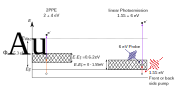
\includegraphics[width=0.85\textwidth]
		{figures/2PPEvsARPES3.pdf}}
		\caption{Depiction of the \gls{2PPE} (left) and LPE (right) excitation process for the model system using the workfunction $\Phi_{Au}$ of \gls{au}. The hatched area depict the elevated states detected above \gls{ef}.
		}
		    \label{2PPEvsARPES}
	\end{figure}
Fig.\,\ref{2PPEvsARPES} depicts the difference between \gls{2PPE} and LPE on a \gls{au} surface, indicated by the workfunction $\Phi_{Au} = 5.3\,\mathrm{eV}$, whereby the hatched areas present the probed regions of the excited states. The clear advantage of LPE is the ability to probe right up and even below the Fermi-level.
For LPE the probe photons, here of $6\,\mathrm{\mbox{eV}}$ photon energy, has a photon energy larger than the workfunction of the probed material. This means the probe can access all electronic states above \gls{ef} and part of the states below \gls{ef}.%\\
	\begin{equation}
	        \label{energybelowef}
	    E\textsubscript{$\mathrm{F}$} - E = h\nu -\Phi > 0
	\end{equation}
With \textTheta \,\,being the workfunction of the material and $h\nu$ the used photon energy of the probe beam, giving us the observable range below \gls{ef}. By increasing the probe energy one can look into lower lying ground states, or by varying the pump energy gain access to a different energy interval of the unoccupied states. Since \gls{LPE} provides the opportunity to probe electrons below \gls{ef}, the excitation by the pump beam can reveal hole states and their decay dynamics. 
        	
        	
\subsection{Au/Fe/MgO(001) Heterostructure System}
    \label{chapHS}
    \begin{wrapfigure}{R}{0.4\textwidth}
		\center{\includegraphics[width=0.38\textwidth]
		{figures/samplelayout.png}}
		\caption{Layout of the sample film thicknesses (left) and three-dimensional visualisation (right). The lateral dimensions of the sample are $9\,\mathrm{mm}$ by $9\,\mathrm{mm}$.}
	    	\label{samplelayout}
	\end{wrapfigure}  
As a model system to study the effects of electron transport, an \gls{fe}-\gls{au} heterostructure on \gls{mgo} was chosen. The \gls{mgo} substrate provides a (001)-crystal surface, which is ideal for epitaxial growth and thus important for sharp crystalline interfaces. This enables to neglect interface scattering contributions in the analysis of electron relaxation dynamics. Furthermore \gls{mgo} has good transmittance for the $800\,\mathrm{\mbox{nm}}$ pump-beam light, because of the $7.8\,\mathrm{eV}$ band gap \cite{NOUROZI20192038}. The dimensions of the \gls{mgo} crystal are $10\,\mathrm{mm}$ by $10\,\mathrm{mm}$ with a thickness of $\pm\,0.02\,\mathrm{mm}$.  The first layer on the \gls{mgo} is a $7\,\mathrm{\mbox{nm}}$ thick, epitaxially grown \gls{fe} film and on top of this a second layer of \gls{au} with varying thicknesses is grown. The \gls{fe}-layer, due to its strong absorption in the visible range, acts in back side pump configuration as an injection layer of 'hot' electrons into the \gls{au}-layer. Those excited electrons propagate through the Fe-Au interface towards the \gls{au}-layer surface and will then be probed out of the \gls{au} surface by a time delayed UV pulse with the photon energy $h\nu_{probe}=6\, \mathrm{eV}$. Laser absorption profile calculation in Sec.\,\ref{CLAPchap} will show  that most of the energy of the pump beam light, in case of back side pump configuration, is absorbed in the \gls{fe}-layer.\\
In case of front side excitation, the pump beam excites directly on the probed \gls{au} surface observing the influence of \gls{fe} as a sink for the electrons by changing the thickness of the \gls{au}-layer. The utilised sample was grown by D. Diesing and J.P. Meyburg from the chemistry department of the university Duisburg-Essen using molecular beam epitaxy (MBE). The sample layout is shown in Fig.\,\ref{samplelayout}. The substrate is a $9\,\mathrm{mm}$ x $9\,\mathrm{mm}$ square of a $0.5\,\mathrm{mm}$ thick \gls{mgo} substrates on which nine different $3\,\mathrm{mm}$ x $3\,\mathrm{mm}$ areas of \gls{fe}/\,\gls{au} layers are grown in a $[001]_{\mathrm{Au}} ||\, [001]_{\mathrm{Fe}} ||\, [001]_{\mathrm{MgO}}$ orientation. The epitaxial growth of the different layers and their pristine interface were demonstrated by Mühge et al. for \gls{mgo}/\,\gls{fe} \cite{Mhge1994} and Dekadjevi et al. for \gls{fe}\,/\,\gls{au} \cite{PhysRevLett.86.5787}. The layers are grown in three rows of different \gls{fe} thicknesses ($7\,\mathrm{nm}$, $15\,\mathrm{nm}$ and $30\,\mathrm{nm}$) and three columns of \gls{au} thicknesses ($5\,\mathrm{nm}$, $15\,\mathrm{nm}$ and $30\,\mathrm{nm}$). Since previous experiments have shown that increasing the \gls{fe} thickness only reduces the injection efficiency of 'hot' electrons, see supplement of Beyazit et al. \cite{beyazit2019}, only the $7\,\mathrm{nm}$ \gls{fe} row of the sample was used for the study reported here. For understanding the dynamics that is being observed, it is important to know the bandstructure of \gls{au} and \gls{fe} explained in Sec.\,\ref{CPEBchap}.


\subsection{Determination of Spatial and Temporal Overlap using Thin Pb Films on Si(111)}

Before starting the \gls{LPE} measurements on the \gls{au} / \gls{fe} / \gls{mgo} samples the light beams were characterised. This was an iterative process of optimisation repeated before almost every measurement. To characterise the light beams in their focal point they were recorded on a \gls{ccd} camera with a resolution of $5.6\,\mathrm{\mu m}$ per pixel. The goal was to focus the beams to the smallest possible diameter, while maintaining a Gaussian shape. The diameter of the $1.55\,\mathrm{eV}$ pump beam diameter was deliberately enlarged to remain larger than the $6\,\mathrm{eV}$ probe beam diameter to ensure homogeneous excitation. Usually the beam diameter was less than $200\,\mathrm{\mu m}$ for the $6\,\mathrm{eV}$ beam. The beams were optimised using the angle and position of the \gls{bbo} crystal and the position of the focusing lens.\\
The beams where analysed with a \gls{ccd} camera determining the full width at half maximum (FWHM) horizontally and vertically from the peak intensity. Both images in Fig.\,\ref{figfrog800} and \ref{figfrog200} are overexposed to illustrate the beam pulse shapes. While the $6\,\mathrm{eV}$ laser beam, see Fig.\,\ref{figfrog200}, has a very sharp Gaussian form, focusing the $1.55\,\mathrm{eV}$ beam distorted the Gaussian form of the laser pulse significantly with some reflexes being visible in Fig.\,\ref{figfrog800}. The distortion and reflexes of the $1.55\,\mathrm{eV}$ pump beam might be due to some of the optical elements used, like the prisms, lenses or attenuator.
\\
To adjust to the \gls{LPE} experimental setup, \gls{pb} was measured with the \gls{ptof} in front side pump / front side probe configuration, as a known system. To prepare the \gls{pb} films on Si(111) a well established routine is being followed. The \gls{pb} film was freshly prepared every morning in ultra high vacuum before starting the experiments \cite{Sandhofer2014}. The substrate was a Si(111) single crystal, that was first annealed to create the 7 x 7 reconstruction by slowly increasing the applied current up to $4.6\,\mathrm{A}$ to heat the Si(111) wafer, while it is being cooled by liquid nitrogen flowing through the manipulator. 
 	\begin{figure}[H]
 	    \begin{minipage}[t]{.44\linewidth}
        	\includegraphics[width=\linewidth]{figures/Frog800nm.png}
			\caption{CCD-camera recording of the $1.55\,\mathrm{eV}$ pump beam in the focal point with a diameter of $212\,\mathrm{\mu m}$ vertically and $180\,\mathrm{\mu m}$ horizontally at FWHM. The black scale is $112\,\mathrm{\mu m}$ large and the colorscale depicts the pixel intensity from 0 to 255.}
			    \label{figfrog800}
		\end{minipage}
			\hspace{.05\linewidth}
		\begin{minipage}[t]{.5\linewidth}
			\includegraphics[width=\linewidth]{figures/layout200nm.png}
			\caption{CCD-camera recording of the $6\,\mathrm{eV}$ probe beam in the focal point with a diameter of $168\,\mathrm{\mu m}$ vertically and $156.8\,\mathrm{\mu m}$ horizontally at FWHM. The black scale is $112\,\mathrm{\mu m}$ large and the colorscale depicts the pixel intensity from 0 to 255.}
			    \label{figfrog200}
		\end{minipage}
	\end{figure}
\noindent
The thermocouple of the manipulator heated up to about $200\,\mathrm{K}$, while the sample reached temperatures of $1000\,\mathrm{K}$, measured by using an infrared thermal imaging camera. Since silicon is a semiconductor, the electronic band gap of about $1.1\,\mathrm{V}$ must first be reached before a current flows, heating the sample \cite{benstreetman1999}. To avoid shattering the wafer, it needed to be heated at a slow and steady rate and without a temperature gradient across the sample. The first point is fulfilled by ramping up the voltage gradually over $45\,\mathrm{min}$ reaching a heating rate of $1\,\mathrm{K}$ every $5\,\mathrm{s}$, the second point of avoiding temperature gradients is only a problem if the sample is not contacting the tantalum sheets, that are holding the sample, evenly. If the tantalum sheets are not consistently contacting the Si-wafer it might break, because of high temperature gradients. This procedure was carried out twice to ensure a good surface quality. 
Next \gls{pb} was evaporated using a Knudsen effusion cell. The same preparation steps as reported in Sandhofer et al.\cite{Sandhofer2014} were used. The \gls{pb} film was flashed for $40\,\mathrm{s}$ with a current of $0.1\,\mathrm{A}$ flowing through the Si(111) wafer to have the right ß - \textsurd3 x \textsurd3 reconstruction.
Fig.\,\ref{figPbcorr} shows a typical photoemission spectrum of \gls{pb}. The count rate of the \gls{ptof} detector is displayed against the kinetic energy of the detected electrons. The black line is the spectrum with just the $6\,\mathrm{eV}$ spectrum, while the red plot is the correlated signal of both beams. The overlap was produced by first aligning the beams through the pinhole and CCD camera and then scanning for the temporal overlap until a correlated signal is found. After finding the spatio-temporal overlap and fine tuning the system the sample holder was changed to the \gls{au} / \gls{fe} / \gls{mgo} sample holder to start with the actual experiments.
 	\begin{figure}[H]
 	    \begin{minipage}[t]{.45\linewidth}
        	\includegraphics[width=\linewidth]{figures/Pbcorr.pdf}
			\caption{Photoemission spectrum of a thin Pb film on Si(111). The black line depicts the $6\,\mathrm{eV}$ probe spectrum and the red line the correlated signal.}
			    \label{figPbcorr}
		\end{minipage}
			\hspace{.075\linewidth}
		\begin{minipage}[t]{.45\linewidth}
			\includegraphics[width=\linewidth]{figures/PBonlypump.pdf}
			\caption{Photoemission spectrum of the $1.55\,\mathrm{eV}$ pump pulse on Pb/Si(001) thin films, same scale as in Fig.\,\ref{figPbcorr} for comparison.}
			    \label{figPbpump}
		\end{minipage}
	\end{figure}
\noindent
The black line in Fig.\,\ref{figPbcorr} shows the unpumped probe spectrum. The lower energy cutoff towards $\mathrm{E}_{kin}$ = $0\,\mathrm{eV}$, the secondary edge, is visible. The Fermi-level determines the sharp drop at $2.2\,\mathrm{eV}$. By using the difference of the secondary edge and the Fermi-level of the unpumped spectrum and Eq.\,\ref{energybelowef} the workfunction $\Theta$\, of the \gls{pb} films on Si(111) was determined to be $4.0\,\pm0.4\,\mathrm{eV}$, which is in agreement with the literature value of $\Theta_{Pb} = 4.00\,\pm0.02\,\mathrm{eV}$ \cite{PhysRev.102.367}. This indicates a well prepared \gls{pb} film. Above $2.2\,\mathrm{eV}$ there are very few counts from multiphoton events. This is a general trend for $6\,\mathrm{eV}$ illumination. The red trace is the correlated signal of the pump and probe beam overlapping both spatially and temporally. The additional intensity above $2.2\,\mathrm{eV}$ when compared to the unpumped probe spectrum comes from two photon photoelectron emission by $6\,\mathrm{eV}$ and $1.55\,\mathrm{eV}$ photons. This is the \textit{time-resolved} effect being analysed. Fig.\,\ref{figPbpump} shows the multiphoton effects of the $1.55\,\mathrm{eV}$ pump beam generated by 3 to 4 photons. These multiphoton effects are depended on the surface conditions and the incident fluence. Higher fluences lead a better contrast of the correlated signal, but to increased multiphoton effects as well, finding a satisfactory spot on the sample reduces the signal from multiphoton effects by the pump beam.

    \subsection{Experimental Configuration}
The chamber allows for pumping and probing from the front side of the sample on the \gls{au} surface, as well as pumping the bottom layer through the transparent substrate from the back side and probing the top layer surface, see Fig.\,\ref{expsetup}. The sample holder is fixed on a movable manipulator, that can adjust the laser beam position on the sample in $10\,\mathrm{\mu m}$ steps. This way all nine different sample thicknesses can be accessed.
	\begin{figure}[H]
	    \center{\includegraphics[trim={0 0 0 0},clip,width=0.9\textwidth]
		{figures/experimentalsetup.pdf}}
		\caption{Experimental sample setup as used in this thesis.}
	    	\label{expsetup}
	\end{figure}
 

       \subsection{Determining the Electronic Start Signal}
            \label{chapDESS}
    \begin{wrapfigure}[21]{tR}{0.5\textwidth}
		\center{\includegraphics[trim={300 135 370 78},clip,width=0.5\textwidth]
		{figures/bias.pdf}}
		\caption{Energy diagram of the sample and detector with a negative bias voltage $U_B$.}
	    	\label{bias}
	\end{wrapfigure}
To determine the energy of the electrons an \gls{ptof} spectrometer is used. The kinetic energy of an electron is linked to its velocity, see Eq.\,\ref{kinenergy}.
    \begin{equation}
        \label{kinenergy}
        \mathrm{E}_{kin} = \frac{ 1 }{ 2 } m_{ e }*v^{ 2 }
    \end{equation}
With $m_{e}$ being the rest mass of the electron.
The velocity $v$ of the electron is calculated by considering the distance it travels from the sample to the detector and dividing it by the time interval between a measured start and stop signal.
    \begin{equation}
        \label{velocity}
        v = \frac{ L }{ t_{stop} - t_{ start }  }
    \end{equation}
With the distance $L$ and the stop signal $t_{stop}$, the electronic signal of the detector when an electron hits the hexagonal wire anode. The start signal $t_{start}$ is given by a photo-diode being hit by a fraction of the laser pulse. The temporal width per energy bin in the spectrometer is $249.94\,\mathrm{ps}$.  To compensate for the travel time of the signal in the cables, the light travelling to the sample surface and the speed of the processor, the start signal for the \gls{ptof} is corrected by a summand \textalpha\,\cite{Lisowski}.
    \begin{equation}
        \label{startsignal}
        t_{start} = n * 249.94\,\mathrm{ps} + \alpha
    \end{equation}
To determine this summand \textalpha\, the fact, that the velocity $v$ of the electron scales quadratic, while the kinetic energy $E_{kin}$ scales linearly, is used. The setup allows for a bias voltage $U_B$ to be applied between the spectrometer and the sample, this bias voltage can be used to accelerate and decelerate the electrons leaving the sample. By recording different spectra with different applied bias voltages, the exact offset \textalpha\, of the $t_{start}$ signal can be determined. The bias voltage $U_{b}$ gives some control over the energy levels the detector can observe as well. In Fig.\,\ref{bias} the Fermi-level and $E$\textsubscript{\textit vac}, the energy needed for an electron to escape the material, of the spectrometer and the sample are shown. A bias voltage $U_{b}$ can now be applied to change \gls{ef} and $E$\textsubscript{\textit vac} with respect to the detector, but not to each other. If the $E$\textsubscript{\textit vac} of the sample is below $E$\textsubscript{\textit vac} of the detector, part of the spectrum will be cut off, because the detector wont be sensitive for it. The spectrometer is permanently grounded, so $U_{b}$ is used to equalise the two $E$\textsubscript{\textit vac}. In the bias series $U_{b}$ now varies and the summand \textalpha\, for the electronic start signal delay is calculated. The electronic start and stop signal delay gets updated by a new bias series, when the experimental setup changes.
\\
Next the data sets get loaded in by a previously written Igor macro, which helped with data analysis. The raw data sets look like the one shown in Fig.\,\ref{raw}. Here the previously determined $t_{start}$ comes into play to set the right energy bins for the conversion of the timing signal to the energy bins. Since the relation of time and energy is not linear, the data needs to be converted using Eq.\,\ref{timeenergy} \cite{Lisowski}.
    \begin{equation}
        \label{timeenergy}
        \frac{ dN }{ dE_{ kin } } = \frac{ dN }{ dt  }*\left\lvert \frac{ dt }{ dE_{ kin } }\right\rvert = \frac{ dN }{ dt  }* \frac{ \left( t - t_{0} \right)^{3} }{ m_{e} * L^{2} } = \frac{ dN }{ dt  } * \sqrt{ \frac{m_{e} * L^{2}}{ 8 }} * E_{kin}^{-\frac{ 3 }{ 2 }}
	\end{equation}
Because the relation between energy and time-of-flight is non-linear, the relation of the size of the bins is not either. With a fixed temporal width of $250\,\mathrm{ps}$ the faster electrons are detected with higher accuracy regarding their energy, because they fall onto narrower but denser energy bins, while the slower electrons are detected in wider energy bins. Since \textDelta E scales non linearly with the flight time it was considered if $dE$\,/\,$dt$ needs to be weighted, when integrating the energy resolved spectrum, but it should not be needed, because the detection probability is already determined by the energy resolved spectrum.



    \subsection{Setting the Relative Time Delay}
        \label{chapSRT}
First, when loading the data into a new Igor file, the length of the drift tube is set to $200\,\mathrm{mm}$ for the calculation of the energy bins, see Sec.\,\ref{chapDESS}. Next the electronic start signal gets adjusted by the value determined in the bias-series. For the measurements discussed here it lies between $14.1\,\mathrm{ns}$ and $18.7\,\mathrm{ns}$. The procedure is the same for every data set and will be discussed briefly on the $5\,\mathrm{nm}$ \gls{au} / $7\,\mathrm{nm}$ \gls{fe} / \gls{mgo} back side pump configuration as an example. The measurements accumulate 100 scans for every pump-probe delay, collecting data with a bin size of $250\,\mathrm{ps}$, to reach satisfactory statistics. The pump-probe spectrum first looks like Fig.\,\ref{raw}. The kinetic energy gets resolved by the time-of-flight spectrometer for every time delay. The 2D-colour plot indicates the photoelectron yield of the detector at every timestep and energy bin. The correlated signal at $t_0$ is not visible, because the induced changes are to small compared to the non-correlated signal in linear photoelectron emission. The correlated signal is found between $3.8$ and $2.3\,\mathrm{eV}$. The high photoelectron yield between $1$ and $2\,\mathrm{eV}$ is the linear photoemission of the $6\,\mathrm{eV}$ probe beam photons.
	\begin{figure}[H]
	    \center{\includegraphics[width=0.9\textwidth]
		{figures/examplespectrum.pdf}}
		\caption{Pump-probe spectrum of the $5\,\mathrm{nm}$ \gls{au} / $7\,\mathrm{nm}$ \gls{fe} / \gls{mgo} back side pump measurement after loading it with the provided Igor file. The colorcode goes from blue (low intensity) over brown to white (high intensity) indicating the measured photoelectron yield. Zero pump-probe delay means a correlated signal.}
	    	\label{raw}
	\end{figure}
\noindent First \gls{t0} is set to the bin with the signal from the electrons with the highest energy, see Fig.\,\ref{timezerofit}, because they arrive at the detector first and are assumed to travel ballistic, and if they travel in a (\textit{super})-diffusive regime, it will be assumed that the scattering rates are constant for all samples giving the same error. Setting \gls{t0} is done by fitting a Gaussian to the distribution of the electrons with the highest energy, found here at a kinetic energy of about $3.85\,\mathrm{eV}$, and setting \gls{t0} to the thereby obtained peak position. 
	\begin{figure}[H]
	    \center{\includegraphics[width=0.9\textwidth]
		{figures/timezerofitupdate.pdf}}
		\caption{Blue: The electrons with the highest kinetic energy around $t_0$ (integrated over $100\,\mathrm{meV}$). They are found at a kinetic energy of $3.85\,\mathrm{eV}$ and red: the Gaussian fit to model the position of time zero. Fitting parameters can be found in the text.}
	    	\label{timezerofit}
	\end{figure}
\noindent To model the Gaussian shape of the electron distribution the \gls{fwhm} of the Gaussian was held at the measured cross-correlation of $84\,\mathrm{fs}$, assuming no broadening by propagation. The offset to account for the background, the amplitude and time offset was varied. The time offset was set to 0 after the variation is done.
The Gaussian fit like shown in Fig.\,\ref{timezerofit} is used, because the probe beam convolves with the electron distribution generated by the pump beam generating a cross-correlation, that is broadened by the Gaussian shape of the pulses. 
Then \gls{ef} needs to be defined as zero to be a reference between the different measurements. Because all measurements with different sample positions had different count rates, an energy below \gls{ef} is chosen, where all measurements are normalised to 1, as will be discussed in Sec.\,\ref{chapNFLF}.
      
      
\newpage      
\section{Experimental Results}
In the experimental results the performed experiments are going to be analysed energy resolved by their energy density $U(E,t)$. First the laser absorption profiles were calculated to understand how the excitation process happens, then $U(E,t)$ was estimated by a Fermi-Dirac distribution modelled before and during excitation. Then after subtracting the background the relative number of holes and electrons could be determined allowing discussion of hole dynamics. The information of the relative number of electrons was increased by weighting the energy to a energy density $U(E,t)$. This allowed discussion of injection efficiencies and relaxation times. Analysis of time independent energy transients revealed a spectral feature and the importance of secondary electrons being generated.
    \subsection{Calculation of Laser Absorption Profile}
        \label{CLAPchap}
This work studies transport mechanisms and relaxation dynamics of laser excited non-equilibrium electrons. In order to characterise the dynamics of these electrons, the process of excitation and detection must be well understood. For this the interaction of the used light beams with the heterostructure was simulated. Thereby gaining insight into the absorption process and its localisation.
For the calculation of the laser absorption profile the program \gls{xop} was used \cite{Laserprog,Dejus1996}. Details on the analysis can be found in Sec.\,\ref{OPDchap}. The program was originally designed to simulate X-ray diffraction in crystals, but it can likewise be used for our laser profiles by amending the necessary data sets. To calculate the absorption depth of the $800\,\mathrm{\mbox{nm}}$ and $200\,\mathrm{\mbox{nm}}$ light beams the program needs several optical constants, which where taken from Weaver for \gls{au} and Palik for \gls{fe} and \gls{mgo} \cite{weaver1981optical2,palik1991handbook}. The procedure from Eschenlohr et al. was used, who simulated a similar combination of constituent thicknesses of \gls{au}/\,Ni/\,Pt/\,Al \cite{Eschenlohr2014}. 



%	\begin{table}[H]
%	    \centering
%		\caption{\gls{xop} inputs FP means front side pump, BP means back side pump}
%		\vspace{3mm}
%		\begin{tabular}{ccc}
%			\gls{au} thickness [nm] & \gls{fe} thickness [nm] & laser geometry \\
%			\hline
%			5 & 7 & \gls{fp} and \gls{bp} \\
%			15 & 7 & \gls{fp} and \gls{bp} \\
%			30 & 7 & \gls{fp} and \gls{bp} \\
%		\end{tabular}
%		    \label{lasercalc}
%	\end{table}
	
The same configurations of the heterostructure were simulated as used in the experiment with $d_{fe} = 7\,\mathrm{nm}$ and $d_{au} = 5,\,15,\,30\,\mathrm{nm}$. The angle of incident for the calculations is $45\,$\textdegree\, and the light polarisation was p-polarised (E-field parallel to the normal of the sample surface), like the experiments performed. The calculations have shown, that the \gls{mgo} substrate does not affect the back side pump light and was therefore omitted. The light intensity (black trace), the absorbed laser power (blue trace) and the change in the absorbed laser power $dP/dz$ (red trace), was plotted against the position in the heterostructure along the surface normal for $30\,\mathrm{\mbox{nm}}$ \gls{au} in back side pump geometry, see Fig.\,\ref{30nmbplaser}. The first $7\,\mathrm{nm}$ are the \gls{fe}-layer. For the square of the light intensity one can observe an exponential decrease with a slight kink right at the \gls{au}\,/\,\gls{fe}-interface.
	 
	\begin{figure}[H]
	    \center{\includegraphics[width=0.9\textwidth]
		{figures/30nmBackpumplaser.pdf}}
		\caption{Laser absorption profile for the $800\,\mathrm{nm}$ on the back side of $30\,\mathrm{\mbox{nm}}$ \gls{au} /\,$7\,\mathrm{\mbox{nm}}$ \gls{fe}, with the first $7\,\mathrm{nm}$ being the \gls{fe} film. The black trace is the intensity of the electric field of the light, the blue trace is the absorbed laser power P(z), normalised to one at the end of the sample, and the red trace shows the differential of the absorbed laser power $dP(z)/dz$. The percent values describe the portion absorbed in the respective constituent and the black line around $15\,\mathrm{nm}$ shows the value of the light intensity dropping to 1/$e$.}
		    \label{30nmbplaser}
	\end{figure}
	\noindent This kink is due to the numerical limitations of the programs calculations. The absorbed laser power P(z) was normalised to 1 at the end of the calculated sample to get relative contributions of the absorption in the constituents. Most of the incident laser power is being absorbed in the $7\,\mathrm{nm}$ \gls{fe}-layer. The linear optical penetration depth $\lambda_{OPD}$ of the $200$ and $800\,\mathrm{nm}$ light was taken at the thickness showing an intensity drop to 1/$e$ of the incident value.
    \begin{equation}
        \label{opd}
        I_{ transmitted } = \frac{ 1 }{ e } = \lambda_{OPD}
    \end{equation}
    \\
% Kleine Bemerkung nebenbei: Wenn das kappa (Imaginaerteil der optischen Konstanten relativ klein , <5, und die Schichtdicke relativ klein ist , < 50 nm, nimmt die Transmission nicht exponentiell sondern fast linear mit der Schichtdicke ab.   )
% Habe ich 2007 auch gestaunt, ist aber so. Hier aber alles so stehen lassen, die Gedankenwelt der Laserphysiker scheint wohl exponentiell zu sein.
This gave different optical penetration depths for the different systems, due to changing optical parameters of \gls{fe} and \gls{au}, but similarities due to the various internal reflections in different sample thicknesses. The results showed, that for $5$ and $15\,\mathrm{nm}$ front side pump $\lambda_{OPD}$ of the $200\,\mathrm{nm}$ light larger is than the \gls{au}-layer thickness $d_{Au}$. This means that the sample is homogeneously exited in the laser spot without creating a diffusion gradient away from the \gls{au} surface.
%For the $800\,\mathrm{\mbox{nm}}$ beam the $\lambda_{OPD}$ is shown in the following table \ref{OPD800}
%\\
%	\begin{table}[H]
%	\centering
%		\caption{Estimated $\lambda_{OPD}$ in nm for the $1.55\,\mathrm{\mbox{eV}}$ beam. FP meaning frontside pump and BP back side pump.}
%				\vspace{4mm}
%		\begin{tabular}{cccc}
%			laser geometry & $5\,\mathrm{\mbox{nm}}$ \gls{au} & $15\,\mathrm{\mbox{nm}}$ \gls{au} & $30\,\mathrm{\mbox{nm}}$ \gls{au} \\
%			\hline
%			\gls{fp} & N/A & N/A & $14.8$ \\
%			\gls{bp} & N/A & N/A & $15.3$ \\
%		\end{tabular}
%		    \label{OPD800}
%	\end{table}
Only for the $30\,\mathrm{\mbox{nm}}$ \gls{au} samples enough of the laser intensity gets absorbed and reflected so that this work can estimate an optical penetration depth for the $1.55\,\mathrm{\mbox{eV}}$ pump beam in front pump of $\lambda_{OPD} = 14.8\,\mathrm{nm}$. If we look at the calculations of the $6\,\mathrm{\mbox{eV}}$ probe beam, see Fig.\,\ref{5nmProbelaser}, we observe much more absorption in \gls{au} even for $5\,\mathrm{\mbox{nm}}$ film thickness, when compared to the $1.55\,\mathrm{\mbox{eV}}$ in front side pump configuration.

	\begin{figure}[H]
	    \center{\includegraphics[width=0.9\textwidth]
		{figures/5nmProbe.pdf}}
		\caption{Laser absorption profile for $200\,\mathrm{nm}$ wavelength on $5\,\mathrm{\mbox{nm}}$ \gls{au} /\,$7\,\mathrm{\mbox{nm}}$ \gls{fe}. The first $5\,\mathrm{nm}$ are the \gls{au} film. With the black trace describing the intensity of the electric field of the light, the blue trace the absorbed laser power $P(z)$ normalised to 1 at the end of the sample and the red trace showing the differential of the absorbed laser power $dP(z)/dz$. The percent values describe the portion absorbed in the respective constituent.}
		    \label{5nmProbelaser}
	\end{figure}
These calculations show where the electrons get excited by the pump and the probe light, respectively. Besides it should be considered that the electrons need to have enough energy to be excited into states above the vacuum energy $E_{vac}$, which requires to overcome the workfunction \textTheta\,$ = E_{vac} - E_{\mathrm{F}}$ of about $5\,\pm0.2\,\mathrm{\mbox{eV}}$ depending on the surface condition. It also needs be close to the \gls{au}\,/\,vacuum interface to escape the metal and make it into the detector. Since the transmission function $T(E)$ is unknown for the \gls{au} / vacuum interface a electronic escape depth of about $\lambda_{PES} = 2\,\mathrm{nm}$ is estimated, taken from Lisowski et al. \cite{Lisowski2004}.
To calculate the ratio of the absorbed pump laser energy with the probed energy density of the correlated signal, the fluence of the $1.55\,\mathrm{\mbox{eV}}$ pump beam was measured right before entering the vacuum chamber. The incident power was measured with a photodiode power sensor. Eq.\,\ref{powermeter} shows the relation of the measured power to the fluence on the sample.\\
\begin{equation}
    \label{powermeter}
    F = \frac{ P\left[ J/s \right] *f_{rep}[s] }{ d_{laserspot} \left[cm^{2} \right] }*c_{loss}\left[\%\right] 
\end{equation}
The fluence $F$ is calculated by taking the measured power $P$ and multiplying it with the repetition rate $f_{rep} = 250\,\mathrm{kHz}$ and dividing by the laser spot diameter $d_{laser}$, that
	\begin{figure}[H]
		\begin{minipage}{.45\linewidth}
		     was determined on the \gls{ccd} camera, see Fig.\,\ref{figfrog800}. Because the pump beam is reflected off one more mirror and gets transmitted through the viewport into the ultra high vacuum chamber a loss of 10\% gets added estimated from the transmission value of the viewport and the reflectance of the used silver coated mirror. Five of the six experiments were conducted using a fluence of $F = 70\,\mathrm{\mu J/cm^{2}}$. For the $5\,\mathrm{\mbox{nm}}$ \gls{au}\,/\,\gls{fe} front side pump experiment the fluence was increased to $F = 100\,\mathrm{\mu J/cm^{2}}$ via reducing the optical attenuation, because $F = 70\,\mathrm{\mu J/cm^{2}}$ was not sufficient to detect a signal.
		\end{minipage}
			\hspace{.075\linewidth}
		\begin{minipage}{.45\linewidth}
			\includegraphics[width=\linewidth]{figures/laserremind.pdf}
			\caption{Laser absorption profile for the $800\,\mathrm{nm}$ pump beam on the surface of $5\,\mathrm{\mbox{nm}}$ \gls{au} /\, $7\,\mathrm{\mbox{nm}}$ \gls{fe} /\, \gls{mgo} in front side pump configuration. The first $5\,\mathrm{nm}$ are the \gls{au} film. The percent values describe the portion absorbed in the respective constituent.}
			    \label{laserremind}
		\end{minipage}
	\end{figure}
\noindent
Knowing the incident fluence on the sample the transmittance, absorbance and reflection of the different sample layouts was calculated. Using the calculated absorption the energy content can be split into the constituents using $P(z)$ of the laser absorption profiles. The absorption of the heterostructure decreases with increasing \gls{au} thickness towards the bulk value of \gls{au}. Back side pumping always shows a higher absorption for the same film thickness of \gls{au}.
	\begin{table}[H]
	    \centering
		\caption{Absorbed fluence of the $1.55\,\mathrm{eV}$ for the different constituents, all values are given in $\mathrm{{\mu J/cm^{2}}}$ }
		\vspace{4mm}
		\begin{tabular}{ccc|cc}
			\gls{au}-layer thickness & \multicolumn{2}{c|}{front side pump}&\multicolumn{2}{c}{back side pump} \\
			\hline
			&Fe&Au&Fe&Au \\
			$5\,\mathrm{\mbox{nm}}$ & 23 & 1.0 & 28 & 2.0 \\
			$15\,\mathrm{\mbox{nm}}$ & 14 &0.9 & 22 & 1.4\\
			$30\,\mathrm{\mbox{nm}}$ & 6.0 & 0.3 & 16 & 1.1\\
		\end{tabular}
    		\label{absorption}
	\end{table}
	
	
Table\,\ref{absorption} shows the different fluences $F$ absorbed in the separate constituents. It is found that the absorbed fluence decreases with increasing \gls{au} film thickness, even in the \gls{fe} layer, which is staying the same size, this effect comes from internal reflection inside the \gls{au}-layer. It is also found, that in \gls{fp} most of the laser fluence is still absorbed inside the \gls{fe}-layer. For back side pumping it is assumed, that the observed signal in the \gls{ptof} is absorbed fluence from the \gls{fe}-layer, since the absorption in \gls{au} is negligible. The back side pump configuration always absorbs more laser fluence of the $1.55\,\mathrm{eV}$ pump beam, because of the good absorption of \gls{fe} and the high reflectivity of \gls{au}. The thicker the \gls{au} film gets the less influence the properties of \gls{fe} have in the heterostructure, while moving towards the bulk constants of \gls{au}.\\ \noindent
In Sec.\,\ref{energydensitychap} the absorbed fluence, that was calculated here, is compared to the energy density found at the time-of-flight detector.


\subsection{Determination of the Time Dependent Energy Density}
    \label{chapEED}
This work makes an attempt to quantify the energy content of the excited electrons. Because there are some unknown variables like the transmission function $T(E)$ of the sample and the detection probability the energy density was first modelled for the system. The sensitivity of \gls{LPE} to the Fermi-level allows the observation of pump induced changes in the electronic distribution around \gls{ef}.
To estimate the energy in the system a photoelectron spectrum before excitation by the pump light was plotted. Then the electron distribution in the vicinity of the Fermi energy was modelled by a Fermi-Dirac distribution to estimate a temperature in the system \cite{H.Ibach2008}.
    \begin{equation}
        \label{fermidiraceq2}
        f(E,T) = \frac{ 1 }{ e^{ E-\mu/ k_{ B  }T }+1}
    \end{equation} 
The Fermi-Dirac distribution function provides the temperature dependent probability of occupancy of energy levels by electrons. In practice the temperature $T$\, was varied and a constant background added to account for the normalisation until the Fermi-Dirac distribution modelled the slope of the Fermi edge. For all measurements a temperature was estimated by fitting the photoelectron spectrum before excitation with a Fermi-Dirac distribution, see Fig.\,\ref{fermifitt0} and Eq.\,\ref{fermidiraceq2}, and then this equilibrium temperature was subtracted from the temperature estimated by a Fermi fit at time zero for a $10\,\mathrm{fs}$ interval during excitation, displayed in Fig.\,\ref{fermifit} \cite{H.Ibach2008}. The fits of the spectrum obtained with the probe pulse arriving before excitation with the pump pulse for $5$ and $15\,\mathrm{nm}$ \gls{au} film thickness in both configurations indicate a temperature of about $400\,\mathrm{K}$, for $30\,\mathrm{nm}$ \gls{au} film thickness the estimated temperature was slightly higher at $460\,\mathrm{K}$. These results might be unexpected since all measurements were carried out at room temperature, but the broadening of the Fermi-level by the pump and the probe pulse was not taken into account. By then subtracting the temperature fitted by a Fermi function modelled for the Fermi-level at time zero a temperature increase of about $45\,\pm10\,\mathrm{K}$ for all the measurements can be estimated. This rise in temperature can be converted into an  amount of energy absorbed by \gls{au} using the specific heat capacity $c$ of \gls{au}.
	\begin{figure}[H]
		\begin{minipage}[t]{.45\linewidth}
			\includegraphics[width=\linewidth]{figures/fermifitt0update.pdf}
			\caption{Photoelectron spectrum at $t_0$ for $5\,\mathrm{nm}$ \gls{au} / $7\,\mathrm{nm}$ \gls{fe} / \gls{mgo} in back side pump / front side probe configuration. The blue dots are the experimental data and the red line the fitted Fermi-function. Fitting parameters can be found in the text.}
        		\label{fermifit}
		\end{minipage}
	\hspace{.075\linewidth}
		\begin{minipage}[t]{.45\linewidth}
			\includegraphics[width=\linewidth]{figures/fermifitbeforet0update.pdf}
			\caption{Photoelectron spectrum at a pump-probe delay of $200\,\mathrm{fs}$ before $t_0$ for $5\,\mathrm{nm}$ \gls{au} / $7\,\mathrm{nm}$ \gls{fe} / \gls{mgo} in back side pump / front side probe configuration. The blue dots are the experimental data and the red line the fitted Fermi-function. Fitting parameters can be found in the text.}
    			\label{fermifitt0}
		\end{minipage}
	\end{figure}
\noindent
 Because the excitation generates non-equilibrium electrons, that have not yet thermalised with the lattice, the specific electronic heat capacity $\gamma_{Au}\,= 0.642\,\mathrm{mJ/mol*K^{2}}$ has to be used. For the purpose of estimating an energy it is assumed, that the electrons are already in thermal equilibrium with each other and they can be described both by a Fermi function and the specific electronic heat capacity.
    \begin{equation}
        \Delta Q = \gamma_{Au} * (T + \Delta T)
    \end{equation}
The difference in heat of the system $\Delta Q$ is given by the specific electronic heat capacity $\gamma_{Au}$, the temperature $T$ of the system and the change in temperature \textDelta T. This gave a molar heat increase of $11.56\,\mathrm{J/mol}$. By considering the spot diameter of the probe beam and a probing depth of about $2\,\mathrm{nm}$, taken from Lisowski \cite{Lisowski2004}, the absorbed fluence in the system can be calculated. To calculate the amount of \gls{au} atoms the heat is distributed between, the probed volume is divided by the volume of the primitive unit cell, which contains four \gls{au} atoms, and multiplied by the Avogadro constant $N_A$ to derive the amount of \gls{au} atoms in the probed volume.
    \begin{equation}
        n_{Au} = \frac{ V_{probe}}{ V_{unit \,cell} } * N_{A} * 4
    \end{equation}
This, multiplied with the molar heat increase, divided by the probed area, gives the absorbed fluence $F$
    \begin{equation}
        F = \frac{ \Delta Q * n_{Au} }{ A_{probe} }
    \end{equation}
The calculation gives an idea about the amount of energy in the system. The error was calculated from the error function of the Fermi-Dirac distribution. It is estimated, that the probed area absorbs about $F = 0.6\,\pm1.2\,\mathrm{\mu J/cm^{2}}$.



       \subsection{Determining the width of the Fermi-distribution function}
            \label{Fermidirac}
            
Since \gls{LPE} probes the area around the Fermi-level a shifting of \gls{ef} was observed making the fitting of \gls{ef} to 0 as a reference to compare the spectra difficult. In order to normalise all spectra without temperature dependent influence of \gls{ef} to the same Fermi-level the width of the Fermi-Dirac distribution was calculated.
The Fermi-Dirac distribution, Eq.\,\ref{fermidiraceq2}, accounts for valance electrons in a metal and was discussed in Sec.\,\ref{chapEED} \cite{H.Ibach2008}.
Fig.\,\ref{fermi1} shows Fermi-Dirac distributions modelled for different temperatures, referencing the energy to the Fermi-level of \gls{au}. The Fermi-Dirac distribution gives an approximation of the broadness of the Fermi-level by the tangent of $f(E,T)$ at \gls{ef} intersecting zero at \gls{ef}$+2k_{B}T$. For the used system the width of the Fermi-Dirac distribution was calculated to be $50\,\mathrm{\mbox{meV}}$ \cite{H.Ibach2008}.
    \begin{figure}[H]
		\center{\includegraphics[width=\textwidth]
		{figures/Fermidirac.pdf}}
		\caption{Several calculated Fermi-Dirac distributions for different temperatures. The dashed blue line is a guide to the eye indicating the tangent used for the width determination of the $300\,\mathrm{K}$ trace.}
	    	\label{fermi1}
	\end{figure}
%	\begin{figure}[H]
%		\center{\includegraphics[width=\textwidth]
%   	\caption{Photoemissionspectra of Ru(001) at different temperatures (black lines), overlain with Fermi-Dirac distribution calculations for those temperatures.\cite{H.Ibach2008}}
%		\label{fermi2}
%	\end{figure}


\newpage
        \subsection{Fermi-Level Fit and Normalisation}
            \label{chapNFLF}
The energy level for normalisation was chosen at $-0.1\,\mathrm{\mbox{eV}}$ to have no temperature dependent effects. Now the results of the particular measurements can be compared amongst each other. For normalisation an average intensity value was calculated from spectra before excitation for each data set.\\
Fig.\,\ref{norm} shows a correlated spectrum of an already normalised data set. There are several features visible in this linear representation. Starting from the left, there is the cutoff of the detector at $E\,-\,E_\mathrm{F}\,= -1.85\,\mathrm{\mbox{eV}}$, which can be manipulated by changing the bias-voltage $U_B$ between the sample and the detector.The energy is reverenced to the Fermi-level \gls{ef} Then the strong increase in signal intensity around $E\,-\,E_\mathrm{F}\,= -1.1\,\mathrm{\mbox{eV}}$ is called the secondary edge. After that we observe the electrons from the s and p-bands in the valence band of \gls{au}, that the probe beam can excite by itself in single photoelectron emission. The declining flank around $E\,-\,E_\mathrm{F}\,= 0\,\mathrm{\mbox{eV}}$ is the Fermi edge, the highest occupied ground states. The pump induced changes are so small, that the excited states from the correlated signal are not visible in the linear representation. This is one of the experimental issues, when finding the temporal overlap. The process of fitting \gls{ef} and the normalisation might have to be repeated, because after fitting the Fermi-level the shifted $-100\,\mathrm{meV}$ needs to be normalised again.
	\begin{figure}[H]
	    \center{\includegraphics[width=0.9\textwidth]
		{figures/norm.pdf}}
		\caption{Linear representation of the  correlated signal at $t_0$ of $5\,\mathrm{{nm}}$ \gls{au} / $7\,\mathrm{{nm}}$ \gls{fe} using the front side pump configuration.The energy transient was normalised to 1 at $E\,-\,E_\mathrm{F}\,= -100\,\mathrm{meV}$}
	    	\label{norm}
	\end{figure}

	\begin{figure}[H]
	    \center{\includegraphics[width=1\textwidth]
		{figures/shiftedontop.pdf}}
		\caption{Linear representation of the normalised correlated signal of all samples. All measurements were conducted with a $7\,\mathrm{nm}$ \gls{fe} layer under the \gls{au} layer.}
    		\label{shifted}
	\end{figure}

	\begin{figure}[H]
		\begin{minipage}[t]{.475\linewidth}
			\includegraphics[width=\linewidth]{figures/insetfitbadupdate.pdf}
			\caption{Linear plot between $-0.6\,\mathrm{\mbox{eV}}$ and $0.6\,\mathrm{\mbox{eV}}$ around the Fermi-level for $15\,\mathrm{\mbox{nm}}$ Au in back side pump geometry. Data points (blue) and fit (red). Fit parameters can be found  in the text.}
        		\label{fitbad}
		\end{minipage}
	\hspace{.05\linewidth}
		\begin{minipage}[t]{.475\linewidth}
			\includegraphics[width=\linewidth]{figures/insetfitbad2update.pdf}
			\caption{Linear plot of the Fermi-edge fit for $15\,\mathrm{\mbox{nm}}$ Au in back side pump geometry. Data points (blue) and fit (red). Fit parameters can be found in the text.}
    			\label{fitbad2}
		\end{minipage}
	\end{figure}
\noindent
In Fig\,\ref{shifted} the difficulty in fitting \gls{ef} can already be seen in. The changing peak\begin{wrapfigure}{tR}{0.5\textwidth}
	    \center{\includegraphics[width=0.5\textwidth]
		{figures/insetfitgoodupdate.pdf}}
		\caption{Linear plot of the Fermi-edge fit for $30\,\mathrm{\mbox{nm}}$ \gls{au} in front side pump geometry. Data points (blue) and fit (red). Fit parameters can be found in the text.}
    		\label{fitgood}
	\end{wrapfigure} height of the spectral feature next to the secondary edge, which is probably differing due to surface conditions, interferes with the fit procedure, Because the fit underestimates the slope of the Fermi-edge for the lower energy values. Because of different surface conditions the spectra sometimes variate in the position of the secondary edge. Fig.\,\ref{fitbad} and Fig.\,\ref{fitbad2} show the fit for \gls{ef} of the $15\,\mathrm{\mbox{nm}}$ \gls{au} measurement in back side pump geometry. The spectral feature starting around $-1\,\mathrm{\mbox{eV}}$, see Fig.\,\ref{fitbad2}, is so pronounced that it might start to merge with the Fermi-edge and this makes it difficult to find an energetic lower boundary for the fit. The fit is a convolution of two functions, a Gaussian with a \gls{fwhm} held at the experimentally determined cross correlation of the two light pulses and the Fermi-Dirac distribution at a temperature of $T = 300\,\mathrm{\mbox{K}}$ with an offset and a constant background, whose parameters get optimised and the Fermi-edge gets set where it converges to the lowest error $\chi^{ 2 }$. The detected spectrum is a convolution of the laser pulses, described by the Gaussian function, and the electronic distribution function at the Fermi-level, characterised by the Fermi-Dirac distribution.
	
The count rates of the measurements vary, but to visualise the difference the Signal to Noise ratio (S/N) was calculated. Taking the ratio between correlated and non-correlated signal above the Fermi-level.
	\begin{table}[H]
	    \centering
		\caption{Signal to Noise ratio}
		\begin{tabular}{cccc}
			laser geometry & $5\,\mathrm{\mbox{nm}}$ \gls{au} & $15\,\mathrm{\mbox{nm}}$ \gls{au} & $30\,\mathrm{\mbox{nm}}$ \gls{au} \\
			\hline
			front side pump & 39.8 & 9.8 & 7.7 \\
			back side pump & 15.4 & 8.0 & 7.9 \\
		\end{tabular}
    		\label{stn}
	\end{table}
Table \ref{stn} shows, that the \gls{stn} ratio has a trend of decreasing, when the sample thickness increases. Along with an increase of the \gls{stn}, when the front side pump geometry is used. This is surprising, since \gls{fp} has the problem of the high reflectance of the p-polarised light $R_{ P }(\phi = 45) = 0.966 \,$at$\,1.5\,\mathrm{\mbox{eV}}$ for \gls{au}, while \gls{fe} reflects much less, with $R_{ P }(\phi = 45) = 0.444 \,$at$\,1.5\,\mathrm{\mbox{eV}}$. Not only does this reduce the absorbed energy density $U(E,t)$ for front side pump, but also leads to multiphoton effects, see Fig.\,\ref{figPbpump}, which make finding a suitable spot for a measurement on the surface a real challenge.

The actual measured photoemission spectrum for $30\,\mathrm{\mbox{nm}}$ \gls{au} in back side pump configuration is shown below in Fig.\,\ref{BP30nonorm}. When comparing it to the spectrum of $5\,\mathrm{\mbox{nm}}$ Au in back side pump configuration, Sec.\,\ref{BGSchap} Fig.\,\ref{setfermi}, it can be seen that the signal for $30\,\mathrm{\mbox{nm}}$ \gls{au} has much less intensity.

%	\begin{figure}[H]
%		\begin{minipage}[t]{.45\linewidth}
%			\includegraphics[width=\linewidth]{figures/FP5noNorm.pdf}
%			\caption{$5\,\mathrm{\mbox{nm}}$ \gls{au}\,/\,$7\,\mathrm{\mbox{nm}}$ \gls{fe} in front side pump /\,front side probe geometry.}
%	    		\label{FP5nonorm}
%		\end{minipage}
%	\hspace{.075\linewidth}
%		\begin{minipage}[t]{.45\linewidth}
%			\includegraphics[width=\linewidth]{figures/BP30noNorm.pdf}
%			\caption{$30\,\mathrm{\mbox{nm}}$ \gls{au}\,/\,$7\,\mathrm{\mbox{nm}}$ \gls{fe} in back side pump /\,front side probe geometry.}
%	    		\label{BP30nonorm}
%		\end{minipage}
%	\end{figure}
	\begin{figure}[H]
        \center{\includegraphics[width=0.9\textwidth]
		{figures/30nmBPnoNormSpectrum.pdf}}
		\caption{Time and energy resolved LPE spectrum for $30\,\mathrm{nm}$ \gls{au} / $7\,\mathrm{nm}$ \gls{fe} / \gls{mgo} in back side pump configuration.}
	    	\label{BP30nonorm}
	\end{figure}
 The time dependent photoemission spectrum , see Fig.\,\ref{BP30nonorm}, with the colour code displaying the intensity count of the detector, shows how much intensity there still is above \gls{ef}$\,= 0$ in single photon photoelectron emission. With dark blue being the lowest counts and going over green,yellow to the threshold value at brown. Values above the threshold are displayed white.
The difference in the \gls{stn} ratio is immediately apparent when looking at the colour of the peak and the time independent background at higher energies.
For the $5\,\mathrm{\mbox{nm}}$ measurements the excited electron signal from the $1.55\,\mathrm{\mbox{eV}}$ plus $6\,\mathrm{\mbox{eV}}$ is one order of magnitude bigger than the background above \gls{ef}, while the linear photoelectron emission of the ground states electrons are between 4 \& 6 orders of magnitudes bigger than the correlated signal.
\newpage
        \subsection{Background Subtraction}
            \label{BGSchap}
            	\begin{figure}[H]
        \center{\includegraphics[width=0.9\textwidth]
		{figures/setfermiedge.pdf}}
		\caption{Time and energy resolved LPE spectrum for $5\,\mathrm{nm}$ \gls{au} / $7\,\mathrm{nm}$ \gls{fe} / \gls{mgo} in back side pump configuration. The red rectangle indicates the energy dependent transient used for background subtraction.}
	    	\label{setfermi}
	\end{figure}
The method \gls{LPE} is sensitive to the dynamics of electrons and holes around or below the Fermi-level \gls{ef}, respectively. For sufficiently thin films, with good \gls{stn} ratio, the probe beam can detect the depopulation of states up to $300\,\mathrm{meV}$ below \gls{ef}, as shown in Fig.\,\ref{BGS}. This gives the opportunity to study the transport phenomena and relaxation dynamics of depopulated ground states in a time resolved manner. To depict these, from here on called hole states or depopulated ground states, visually and to make the analysis of them more straight forward the time independent background was subtracted from all data sets. This was done by taking an average value, before excitation, at each energy bin and subtract that at every time delay. After that the background gets subtracted by pulling a random chunk before excitation, see Fig.\,\ref{setfermi}. For good statistics the time window was set to $100\,\mathrm{fs}$, starting $200\,\mathrm{fs}$ before excitation and the outlier was avoided. As long as the time window avoids outliers in the time independent background, the size of \textDelta $t$  does not play a role.

%	\begin{figure}[H]
%		\begin{minipage}[t]{.45\linewidth}
%			\includegraphics[width=\linewidth]{figures/NoBGS.pdf}
%			\caption{normalised time dependent energy resolved spectrum for $5\,\mathrm{\mbox{nm}}$ Au in BP configuration.}
%			\label{NoBGS5BP}
%		\end{minipage}
%	\hspace{.075\linewidth}
%		\begin{minipage}[t]{.45\linewidth}
%			\includegraphics[width=\linewidth]{figures/BGS5BP.pdf}
%			\caption{Background subtracted time dependent energy resolved spectrum for $5\,\mathrm{\mbox{nm}}$ Au in BP configuration. In the colour scale blue means negative change, white equals zero and red are positive changes}
%			\label{BGS5BP}
%		\end{minipage}
%	\end{figure}

\noindent	Every time delay gets subtracted by the pulled chunk before excitation using the following command in Igor Pro 6:
    \begin{equation}
        \label{eqBGS}
    TOF2D\_en\_001\left[ \,\right]\left[\,  \right]-=BGS040\_060\left[ q \right]
    \end{equation}\\
With the first being the name of the matrix of the data and the second the column vector of the time independent background. The hole dynamics becomes visible and the Fermi-level can be fine tuned to the point, where holes and electrons cancel each other out, within a $0.1\,\mathrm{eV}$ window. 
	\begin{figure}[H]
	    \center{\includegraphics[width=0.9\textwidth]
		{figures/BGS.pdf}}
		\caption{2D plot of the background subtracted spectrum for $5\,\mathrm{nm}$ \gls{au} / $7\,\mathrm{nm}$ \gls{fe} / \gls{mgo} in back side pump configuration. Red intensity is above zero, while blue is below. The black lines are guides to the eye for the Fermi-level and $t_0$}
	    	\label{BGS}
	\end{figure}
The colour plot of the background subtraction must be correctly understood, see Fig.\,\ref{BGS}. The mixed red and blue intensity dots at energies $<$\, \gls{ef} is the noise of the measurement.  Then the transition into the white above is due to the reduction of signal intensity but not the Fermi-level, which often lies a bit lower. At zero time delay the absorbed energy of the $1.55\,\mathrm{\mbox{eV}}$ pump pulse is spread evenly over all available excited states. With increasing time a lot of the energy is transferred into lower energy states by scattering processes with ground state electrons, creating a secondary electron of lower energy, about half the initial energy. The small line at $-400\,\mathrm{\mbox{fs}}$ is a measurement error. Below the Fermi-edge a bit after excitation, a reduction in intensity is visible. This reduced intensity is caused by unoccupied ground states, left behind by the excitation processes. These hole states decay over about $500\,\mathrm{\mbox{fs}}$ as visible in Fig.\,\ref{BGS}.

\subsection{Relative Number of Electrons and Holes}
    \label{chapRNEH}
For the energy resolved analysis, an Igor routine is then used to extract the time independent energy resolved transients. Fig.\,\ref{timedep2} shows an example for the first transient, that is pulled via a script, further explained and added in the appendix \ref{chapAp}. These transients are saved as a column vector for every $5\,\mathrm{fs}$, so every data point. Different resolutions of taking 5, 10, 20 and $ 50\,\mathrm{fs}$ were analysed in order to estimate the limits of the resolution but the statistics for $5\,\mathrm{fs}$ was already enough to observe any feature.


		\begin{figure}[H]
	    \center{\includegraphics[width=0.9\textwidth]
		{figures/timedep.pdf}}
		\caption{Energy dependent spectrum at time zero.}
	    	\label{timedep2}
	\end{figure}

	\begin{figure}[H]
	    \center{\includegraphics[width=0.9\textwidth]
		{figures/bins.pdf}}
		\caption{Energy dependent spectrum of time zero. Summed up in $100\,\mathrm{meV}$ bins for computational reasons.}
	    	\label{bins}
	\end{figure}
The next steps are checked by hand calculation as well. After storing all transients, a script, found in the appendix\,\ref{chapAp}, is then run for analysis. First it sums the $5\,\mathrm{meV}$ bins up into $100\,\mathrm{meV}$ bins to make the data easier to be handled. As shown in Fig.\ref{bins}.
To better describe the dynamics of the electrons and holes, the same analytic method as Lisowski et al. reported on \gls{LPE} measurements on Ru(001) was used. First the relative number of electrons and holes around \gls{ef} was calculated \cite{Lisowski2004}.
   
    \begin{equation}
        \label{releeq}
        n_{ \pm } = \int\limits_{0}^{\pm0.3\,\mathrm{eV}} I(E,t) dE
    \end{equation}
     \newline
   
   
    With $n_{\pm}$ being the relative number of electrons or holes and $I(E,t)$ the amount of events detected in the time-of-flight spectrometer with each count corresponding to a single electron hitting the detector.\\
    In order to analyse the various energy states and further find the limits of the data set the upper bound of the integral was varied from $E - E_{\rm{F}}=0$ to $\pm\, 0.6\,\mathrm{\mbox{eV}}$. Fig.\,\ref{EandH5BP} shows that most of the electron and hole dynamics do not appear at time zero, it takes a few ten femtoseconds to build up the intensity. Here all different integral bounds are shown to stress the point, that in the relative distribution most of the observed electrons and holes reside $\pm\,200\,\mathrm{\mbox{meV}}$ around the Fermi-level. When multiplying the relative number of holes with $-1$ and omitting the higher energies, the symmetry of the electrons and holes become very apparent. Fig.\,\ref{EandH5BPsym} features the relative number of electrons and holes integrated over the indicated upper bound. The integration is done in $100\,\mathrm{meV}$ bins and the Fermi-edge here is defined as the bin, where the excited electron signal and the reduction of signal by hole states cancel each other out to a zero baseline. 
	\begin{figure}[H]
		\center{\includegraphics[width=0.9\textwidth]
		{figures/EandH5BP.pdf}}
		\caption{Electrons and holes for $5\,\mathrm{nm}$ \gls{au} / $7\,\mathrm{nm}$ \gls{fe} / \gls{mgo} in back side pump configuration. Black and blue: Electrons, gold and red: Hole states.}
    		\label{EandH5BP}
	\end{figure}
    	\begin{figure}[H]
			\includegraphics[width=0.9\textwidth]{figures/EandH5BPsymImproved.png}
			\caption{Relative number of electrons and holes for $5\,\mathrm{nm}$ \gls{au} / $7\,\mathrm{nm}$ \gls{fe} / \gls{mgo} in back side pump configuration. Black: Electrons, Red: Hole states}
			\label{EandH5BPsym}
        \end{figure}
 The same detection probability for holes and electrons are assumed around \gls{ef}. If the increased noise level of hole dynamics is set  aside, the comparison reveals that the relative number of electrons and holes, displayed in Fig.\,\ref{EandH5BPsym}, are almost identical.
The increased noise of the holes origins from the uncorrelated probe signal, which is five orders of magnitude bigger than the correlated signal. Both electrons and holes decay at the same rates. It is interesting to see, that despite integrating over an energy window three times the size, most electrons and holes are localised within the first $100\,\mathrm{meV}$.
    	\begin{figure}[H]
		\begin{minipage}[t]{.55\linewidth}
			\includegraphics[width=\linewidth]{figures/relativnumberFP.pdf}
			\caption{Relative number of electrons and holes for $5\,\mathrm{nm}$ \gls{au} / $7\,\mathrm{nm}$ \gls{fe} / \gls{mgo} in front side pump configuration. Black: Electrons, Red: Hole states, Green: Fermi-level.}
			\label{relativeFP}
		\end{minipage}
		\hspace{.075\linewidth}
		\begin{minipage}{.375\linewidth}
		 This analysis was performed on the $5\,\mathrm{nm}$ \gls{au} /\, $7\,\mathrm{nm}$ \gls{fe} /\, \gls{mgo} front side pump /\, front side probe measurement as well, see Fig.\,\ref{relativeFP}. In front side pump / front side probe the identification of the reduction of signal is much less strait forward. The signal depletion is now also smaller and not of the same size as the corresponding electron energy.
		\end{minipage}
		\end{figure}
  \noindent For $15\,\mathrm{nm}$ \gls{au} / $7\,\mathrm{nm}$ \gls{fe} in the back side pump measurement, see Appendix \ref{chapAp}, the dynamic is slightly visible, but not distinguishable from background noise. In the rest of the measurements no depletion of ground state signal can be discerned from the noise.
Even if the used approach is not sensitive enough, the excitation process has to create the same number of holes like the observed excited electrons. The holes are less mobile than electrons and have a smaller velocity, because they move by electrons filling a vacant spot in the valence band. $5\,\mathrm{\mbox{nm}}$ \gls{au} in both back and front side pump geometry showed observable depletion of ground states. Thicker \gls{au} films do not show these hole states above the noise, because they have a to low signal to noise ratio, as shown in table\,\ref{stn}.
\\
%        \subsection{Hole Dynamics}
%           \label{HDchap}
%A hole is the absence of an electron in the valence band. In every two photon photoemission spectroscopy holes are created by the pump beam, but in most cases the excited non-equilibrium electrons are in the focus of interest and the created holes do not get observed. Holes are less mobile than electrons and have a smaller velocity, because they move by electrons filling the vacant spot in the valence band. Because of the screening of the positive charge of holes and the high number of electrons in the valance band, holes are difficult to be observed.
To now further analyse the electron dynamics, they get weighted by energy, as Lisowski et al. performed in their work \cite{Lisowski}.


    \subsection{Calculation of the Energy Density in the System}
        \label{chapED}
By weighting the energy of the electrons the information increases from a relative amount of excited electrons and holes to an amount of energy deposited in the probed area during a certain time step \cite{Lisowski2004}. Lisowski has shown, that in order to relate the amount of energy deposited in a system with the intensity at the detector a proportionality factor needs to be incorporated \cite{Lisowski}.
\\
The electronic energy density $U(E,t)$ of an electron distribution
   \begin{equation}
        \label{eldistribution}
        N(E) = f(E,T) * D(E)
    \end{equation}
in a solid with the density of states $D(E)$ and the distribution function $f(E,T)$ is given by
    \begin{equation}
        \label{energydensitystart}
        U_{el} = \int\limits_{ 0}^{ \infty }{ N(E)\, E \,dE} \hspace{5mm}.
    \end{equation}
Lisowski then shows that the intensity $I_{PES}$ being measured is related to the electronic escape depth $\lambda_{PES}$ and a proportionality factor \textalpha\,. This proportionality factor allows the quantitative analysis of the results \cite{Lisowski}. For \gls{au} the electronic escape depth $\lambda_{PES}$ is $2\,\mathrm{nm}$ taken from Lisowski et al. \cite{Lisowski2004}. It is complicated to give the exact value of $\lambda_{PES}$, because the transmission function $T(E)$, the probability of a photoelectron leaving the sample into vacuum, is unknown and must be estimated.
\begin{equation}
    \label{alpha}
I_{PES} (E) = \frac{ \alpha }{ \lambda_{PES} } * f(E,T) * D(E)
\end{equation}
Because $f(E,T)$ and $D(E)$ are unknown above the Fermi-level $E_{\mathrm{F}}$ the proportionality factor \textalpha\,is calculated using a value $E_{\mathrm{1}} < E_{\mathrm{F}}$.

\begin{equation}
\alpha = \frac{I_{PES}(E_{1})}{\lambda_{PES}*f(E_{1},T)*D(E_{1})}
\end{equation}
Here $f(E_1,T)$ is assumed to be one, with $E_1$ far enough away from the Fermi-level and the density of states $D(E_1)$ taken from calculation \cite{Papaconstantopoulos2015}. Then Eq.\,\ref{energydensitystart} and Eq.\,\ref{alpha} are combined and a factor two is added to account for the simultaneously created holes.
    \begin{equation}
        \label{energydensity}
        U(E,t) = \frac{ 2 }{ \alpha * \lambda_{PES} }\int\limits_{E\textsubscript{\textit F} = 0}^{ 1.6\,\mathrm{eV} }{ I(E,t)\, \left\lvert E \right\rvert \,dE}
    \end{equation}
Since the spot size and overlap changes between measurements, the probed area is taken into account as well. By dividing the amount of energy through the probed area a comparable energy density $U(E,t)$ is calculated. Since the detector measures the electron energy in eV the data gets converted into joule by multiplying with the elementary charge to be comparable to the laser irradiation.
	\begin{figure}[H]
	    \center{\includegraphics[width=0.9\textwidth]
		{figures/MitFormel.pdf}}
		\caption{Energy density plot over the entire measurement time of $5\,\mathrm{nm}$ \gls{au}\,/\,$7\,\mathrm{nm}$ \gls{fe} in back side pump configuration, different colours describe different integral bounds. Measured at a $1.55\,\mathrm{eV}$ pump beam fluence of $70\,\mathrm{\mu J/cm^2}$.}
	    	\label{5BP}
	\end{figure}
	
	        \subsection{Energy Density}
            \label{energydensitychap}
This section is devoted to the analysis of the data under the aspect of the amount of energy that is shone onto the system by the pump beam, then excites electrons that start to propagate across the heterostructure, and the amount of energy then detected through the probe beam. The comparisons will be made between the energy densities U($E,t$) of the experiments for different \gls{au} thicknesses $d_{Au}$ and configurations. At appropriate points the energy densities were normalised at $0.1\,\mathrm{\mbox{eV}}$ below \gls{ef}.

The energy density $U(E,t)$ calculated in Eq.\,\ref{energydensity} has the unit $\mathrm{{eV}}$, while the incident fluence was calculated in $\mathrm{{\mu J/cm^{2}}}$. Therefore all plots were multiplied by the coulomb constant and divided by the area of the probe beam $A_{Probe}$.
The following section compares $U(E,t)$ for the three \gls{au} thicknesses, $5\,\mathrm{{nm}}$,$15\,\mathrm{{nm}}$ and $30\,\mathrm{{nm}}$, in front side pump /\, front side probe and back side pump /\, front side probe geometry.
\begin{figure}[H]
	    \center{\includegraphics[width=0.9\textwidth]
		{figures/5nmFPcorr.pdf}}
		\caption{Energy integrated, time dependent transients from $E_{\rm{F}}$ to $1.5\,\mathrm{{eV}}$ for $5\,\mathrm{{nm}}$ \gls{au} / $7\,\mathrm{{nm}}$ \gls{fe} using the front side pump /\, front side probe configuration. Measured at a $1.55\,\mathrm{eV}$ pump beam fluence of $100\,\mathrm{\mu J/cm^2}$.}
	    	\label{5FP}
	\end{figure}
\noindent
When plotting the energy density $U(E,t)$ with the pump-probe delay, see Fig.\,\ref{5BP}, the temporal evolution of the energy density can be seen. The different curves describe different limits for the energy integration and the area between the curves is the amount of energy deposited into electrons with the corresponding energies, e.g. for $\hat{E} = 1.5\,\mathrm{eV}$ its $U(E,t)$ of all hot electrons with an energy above $E-E{\mathrm{\textsubscript F}} = 1.0\,\mathrm{eV}$. The direct comparison between front side pump /\, front side probe and back side pump /\, front side probe, in Fig.\,\ref{5FP} and \ref{5BP}, with the $5\,\mathrm{nm}$ \gls{au} /\, $7\,\mathrm{nm}$ \gls{fe} /\, \gls{mgo} experiments, shows the total measured energy density $U(E,t)$ measured at its peak is twenty times higher for the back side pump measurement. In the front side pump measurements, the electrons are uniformly distributed over the different energies above \gls{ef}, because we probe the area of excitation and therefore the probed electrons do not experience propagation effects. After the initial excitation the electrons do not seem to excite secondary electrons in the probed area. The electrons propagate away from the probed area and the inelastic scattering with 'cold' electrons can not be observed. If a comparison is drawn with the back side pump experiment, the relaxation dynamic behaves a lot different. By the time the electrons get detected, after propagating through the \gls{au}-layer, the electronic distribution is already redistributed towards lower energies. This indicates, that the electrons already started to scatter inelastically with the 'cold' ground state electrons generating secondary electrons. These secondary electrons receive about half the energy of the hot electrons putting them in an energy range of 0 to $0.7\,\mathrm{eV}$ above \gls{ef}. The energy in the system for $5\,\mathrm{nm}$ \gls{au} in back side pump increases after excitation to a value $U(E,t) = 0.08\,\mathrm{\mu J/cm^2}$ higher than before excitation. By using the same way the energy density was estimated by the increase of temperature observed in the Fermi-level, the temperature can be estimated by the increase in energy density at later times.
\begin{equation}
    \label{eqtempph}
\Delta T_{el+ph} = \frac{ \Delta F * A_{probed} }{ c_{Au} }
\end{equation}
\\
\noindent With the specific heat capacity of \gls{au} $c_{Au} = 128\,\mathrm{J/(kg*K^2)}$ giving a temperature increase of $0.21\,\mathrm{K}$ assuming the electrons are equilibrated with the phonons. When just considering the electronic temperature, the specific heat capacity \textgamma$_{Au}$\, for the electrons of \gls{au}.
\begin{equation}
    \label{eqtempel}
    \Delta T_{el} = \frac{ \Delta F * A_{probed} }{ \gamma_{Au} * n * T }
\end{equation}
\\
Using the electronic heat capacity from Eq.\,\ref{eqtempel} the change in temperature is T = $15\,\mathrm{K}$. Only for the $5\,\mathrm{nm}$ \gls{au} back side pump experiment could a lasting increase in $U(E,t)$ during the measurement time of $2\,\mathrm{ps}$ be detected.
	\begin{figure}[H]
		\begin{minipage}[t]{.45\linewidth}
			\includegraphics[width=\linewidth]{figures/15nmFPcorr.pdf}
			\caption{Energy integrated, time dependent transients from $E_{\rm{F}}$ to $1.5\,\mathrm{{eV}}$ for $15\,\mathrm{{nm}}$ \gls{au}\,/\,$7\,\mathrm{{nm}}$ \gls{fe} using the front side pump /\,front side probe configuration. Measured at a $1.55\,\mathrm{eV}$ pump beam fluence of $70\,\mathrm{\mu J/cm^2}$.}
	    		\label{15nmFPnoNorm}
		\end{minipage}
	\hspace{.075\linewidth}
		\begin{minipage}[t]{.45\linewidth}
			\includegraphics[width=\linewidth]{figures/15nmBPcorr.pdf}
			\caption{Energy integrated, time dependent transients from $E_{\rm{F}}$ to $1.5\,\mathrm{{eV}}$ for $15\,\mathrm{{nm}}$ \gls{au}\,/\,$7\,\mathrm{{nm}}$ \gls{fe} using the back side pump / front side probe configuration. Measured at a $1.55\,\mathrm{eV}$ pump beam fluence of $70\,\mathrm{\mu J/cm^2}$.}
    			\label{15nmBPnoNorm}
		\end{minipage}
	\end{figure}
\noindent
	\begin{figure}[H]
		\begin{minipage}[t]{.45\linewidth}
			\includegraphics[width=\linewidth]{figures/30nmFPcorr.pdf}
			\caption{Energy integrated, time dependent transients from $E_{\rm{F}}$ to $1.5\,\mathrm{{eV}}$ for $30\,\mathrm{{nm}}$ \gls{au}\,/\,$7\,\mathrm{{nm}}$ \gls{fe} using the front side pump /\, front side probe configuration. Measured at a $1.55\,\mathrm{eV}$ pump beam fluence of $70\,\mathrm{\mu J/cm^2}$.}
	    		\label{30nmFPnoNorm}
		\end{minipage}
	\hspace{.075\linewidth}
		\begin{minipage}[t]{.45\linewidth}
			\includegraphics[width=\linewidth]{figures/30nmBPcorr.pdf}
			\caption{Energy integrated, time dependent transients from $E_{\rm{F}}$ to $1.5\,\mathrm{{eV}}$ for $30\,\mathrm{{nm}}$ \gls{au}\,/\,$7\,\mathrm{{nm}}$ \gls{fe} using the back side pump /\, front side probe configuration. Measured at a $1.55\,\mathrm{eV}$ pump beam fluence of $70\,\mathrm{\mu J/cm^2}$.}
	    		\label{30nmBPnoNorm}
		\end{minipage}
	\end{figure}
\noindent
The time resolved energy density $U(E,t)$ for the remaining experiments of 15 and $30\,\mathrm{nm}$ \gls{au} both with the same \gls{fe} thickness of $d = 7\,\mathrm{nm}$ in front and back side pump configuration, shown in Fig.\,\ref{15nmFPnoNorm}-\ref{30nmBPnoNorm}, use a $1.55\,\mathrm{eV}$ pump beam fluence of $70\,\mathrm{\mu J/cm^2}$. The $30\,\mathrm{nm}$ \gls{au} front side pump measurement decays similar to the $5\,\mathrm{nm}$ \gls{au} front side pump measurement. On the other hand the $15\,\mathrm{nm}$ \gls{au} front side pump measurement, see Fig.\,\ref{15nmFPnoNorm}, decays less symmetrical, because the electrons with the energy of $0.1\,\mathrm{eV}$ do not decay as fast compared to the other measurements. In back side pump the measurements all have the same form with low energy electrons having longer life times than the higher energetic ones. The thicker films decay faster as will be discussed in Sec.\,\ref{chapR}.
 One can compare the incident laser power, that is absorbed by the constituent, see Sec.\,\ref{CLAPchap}, with the energy that the probe beam observes at time zero. This percentage gives an interpretation of the amount of energy lost during transport. Table\,\ref{tabledensity} displays the peak energy density $U(E,t)$ for each measurement, this does not always coincide with $t_0$, as later discussed in Sec.\,\ref{chapR}.
 	    \begin{table}[H]
	    \centering
		    \caption{Energy density at time zero}
		    \vspace{3mm}
		    \begin{tabular}{ccc}
			    \gls{au} thickness [nm] & front side pump [$\mathrm{\mu J/cm^{2}}$] & back side pump [$\mathrm{\mu J/cm^{2}}$] \\
		    	\hline
		    	5 & 0.07 & 1.48 \\
		    	15 & 0.15 & 0.09 \\
		    	30 & 0.17 & 0.60 \\
		    \end{tabular}
		        \label{tabledensity}
        \end{table}
For front side pump the energy density $U(E,t)$ detected increases with increasing film thickness, see table\,\ref{tabledensity}. The $5\,\mathrm{nm}$ \gls{au}\,/\,$7\,\mathrm{nm}$ \gls{fe} front side pump measurement was performed with $F = 100\,\mathrm{\mu J/cm^{2}}$, while all other only used $F = 70\,\mathrm{\mu J/cm^{2}}$. The values for back side pumping are harder to interpret, because $15\,\mathrm{nm}$ \gls{au} shows a lower energy density than expected. The detected energy density should decrease compared to $d_{Au} = 5\,\mathrm{nm}$, but not stronger than $d_{Au} = 30\,\mathrm{nm}$. The values are mostly lower, than the estimated energy density of $U = 0.6\,\pm1.2\mathrm{\mu J/cm^2}$ but within the error from the Fermi-Dirac distribution, see Sec.\,\ref{chapEED}. Only $5\,\mathrm{nm}$ \gls{au} / $7\,\mathrm{nm}$ \gls{fe} in back side pump configuration shows a higher energy density. The incident laser power absorbed by the constituents, see Sec.\,\ref{CLAPchap}, is compared to the peak energy density that the \gls{ptof} measures. This ratio, shown in table\,\ref{injectable} evaluates the energy loss between the excitation by the pump pulse and the detection by the probe pulse.
 	    \begin{table}[H]
	    \centering
		    \caption{Percentage of absorbed pump fluence detected by the p-e TOF}
		    \begin{tabular}{ccc}
			    \gls{au} thickness [nm] & front side pump & back side pump \\
		    	\hline
		    	5 & 7.0\,\% & 5.3\,\% \\
		    	15 & 17\,\% & 0.4\,\% \\
		    	30 & 56\,\% & 3.8\,\% \\
		    \end{tabular}
		        \label{injectable}
        \end{table}
The laser absorption calculations have shown a decreasing energy content in \gls{au} with increasing film thickness. For front side pump the detection finds a contrary trend of increasing energy density with increasing film thickness, leading to over half the absorbed energy being probed again by the detector. For thinner films of 15 and $5\,\mathrm{nm}$ only a fraction of 17 and $7\,\%$, respectively, is observed at the detector. In back side pump the highest percentage of absorbed fluence detected by the \gls{ptof} is the $5\,\mathrm{nm}$ \gls{au} measurement with $5.3\,\%$, where the electrons have the shortest propagation path after the injection from the \gls{fe}/\gls{au} interface. The thicker films of $15$ and $30\,\mathrm{nm}$ \gls{au} show a reduced detection ratio of $0.4$ and $3.8\,\%$. The ratio of observed energy density is always lower for back side pump.

\subsubsection{Relaxation times}
    \label{chapR}
Because the \gls{stn}-ratio differs widely between the performed experiments, see Sec.\,\ref{chapNFLF}, the data sets were normalised at a point independent of the temperature dependence of the Fermi-level. The broadness of the Fermi-level was calculated in Sec.\,\ref{Fermidirac} and $E - E_\mathrm{F} = -0.1\,\mathrm{eV}$ was chosen as a reference, that is arbitrarily set to 1. The Fig.\,\ref{5nmFPNorm}-\ref{30nmBPNorm} depict the energy density before and after excitation by the pump pulse, first there is a sharp rise of energy density at \gls{t0}, when the pump pulse deposits the energy into the \gls{fe}-layer for back side pump or the \gls{au}-layer for front side pump. In case of back side pump the energy gets transferred into the $0.2\,\mathrm{eV}$ above the Fermi-level within the first $300\,\mathrm{fs}$, see Fig\,\ref{5nmBPNorm},\,\ref{15nmBPNorm} and\,\ref{30nmBPNorm}. It slowly falls off while the electrons relax and transport away from the probed area. 
	\begin{figure}[H]
		\begin{minipage}[t]{.45\linewidth}
			\includegraphics[width=\linewidth]{figures/FPtime.pdf}
			\caption{Energy integrated, time dependent transients from $E_{\rm{F}}$ to $E - E_\mathrm{F} = 1.5\,\mathrm{{eV}}$ for $5\,\mathrm{{nm}}$ \gls{au}\,/\,$7\,\mathrm{{nm}}$ \gls{fe} using the front side pump /\, front side probe configuration normalised to $-0.1\,\mathrm{{eV}}$. Focused around time zero.}
	    		\label{FPtime}
		\end{minipage}
	\hspace{.075\linewidth}
		\begin{minipage}[t]{.45\linewidth}
			\includegraphics[width=\linewidth]{figures/BPtime.pdf}
			\caption{Energy integrated, time dependent transients from $E_{\rm{F}}$ to $E - E_\mathrm{F} = 1.5\,\mathrm{{eV}}$ for $5\,\mathrm{{nm}}$ \gls{au}\,/\,$7\,\mathrm{{nm}}$ \gls{fe} using the back side pump /\, front side probe configuration normalised to $-0.1\,\mathrm{{eV}}$. Focused around time zero.}
	    		\label{BPtime}
		\end{minipage}
	\end{figure}
\noindent
Fig.\,\ref{FPtime} shows the energy density $U(E,t)$ for the first $200\,\mathrm{fs}$ before and after excitation. The time it takes to reach the peak of the energy density is for front side pump ,the order of the cross-correlation of the two pulses. While in front side pump the peak energy density reached is around time zero, the point in time where the electrons with the highest kinetic energy reach the detector, the back side pumped measurement takes 20, 30 and 40 fs for 5, 15 and 30\,nm respectively longer to build up the maximum intensity.
	\begin{figure}[H]
		\begin{minipage}[t]{.45\linewidth}
			\includegraphics[width=\linewidth]{figures/5nmFPNorm.pdf}
			\caption{Energy integrated, time dependent transients from $E_{\rm{F}}$ to $E - E_\mathrm{F} = 1.5\,\mathrm{{eV}}$ for $5\,\mathrm{{nm}}$ \gls{au} in the front side pump configuration normalised to $-0.1\,\mathrm{{eV}}$.}
	    		\label{5nmFPNorm}
		\end{minipage}
	\hspace{.075\linewidth}
		\begin{minipage}[t]{.44\linewidth}
			\includegraphics[width=\linewidth]{figures/5nmBPNorm.pdf}
			\caption{Energy integrated, time dependent transients from $E_{\rm{F}}$ to $E - E_\mathrm{F} = 1.5\,\mathrm{{eV}}$ for $5\,\mathrm{{nm}}$ \gls{au} in the back side pump configuration normalised to $-0.1\,\mathrm{{eV}}$.}
	    		\label{5nmBPNorm}
		\end{minipage}
	\end{figure}
	\begin{figure}[H]
		\begin{minipage}[t]{.44\linewidth}
			\includegraphics[width=\linewidth]{figures/15nmFPNorm.pdf}
			\caption{Energy integrated, time dependent transients from $E_{\rm{F}}$ to $E - E_\mathrm{F} = 1.5\,\mathrm{{eV}}$ for $15\,\mathrm{{nm}}$ \gls{au} in the front side pump configuration normalised to $-0.1\,\mathrm{{eV}}$.}
	    		\label{15nmFPNorm}
		\end{minipage}
	\hspace{.075\linewidth}
		\begin{minipage}[t]{.44\linewidth}
			\includegraphics[width=\linewidth]{figures/15nmBPNorm.pdf}
			\caption{Energy integrated, time dependent transients from $E_{\rm{F}}$ to $E - E_\mathrm{F} = 1.5\,\mathrm{{eV}}$ for $15\,\mathrm{{nm}}$ \gls{au}in the back side pump configuration normalised to $-0.1\,\mathrm{{eV}}$.}
	    		\label{15nmBPNorm}
		\end{minipage}
	\end{figure}
	\begin{figure}[H]
		\begin{minipage}[t]{.44\linewidth}
			\includegraphics[width=\linewidth]{figures/30nmFPNorm.pdf}
			\caption{Energy integrated, time dependent transients from $E_{\rm{F}}$ to $E - E_\mathrm{F} = 1.5\,\mathrm{{eV}}$ for $30\,\mathrm{{nm}}$ \gls{au} in the front side pump configuration normalised to $-0.1\,\mathrm{{eV}}$.}
	    		\label{30nmFPNorm}
		\end{minipage}
	\hspace{.075\linewidth}
		\begin{minipage}[t]{.44\linewidth}
			\includegraphics[width=\linewidth]{figures/30nmBPNorm.pdf}
			\caption{Energy integrated, time dependent transients from $E_{\rm{F}}$ to $E - E_\mathrm{F} = 1.5\,\mathrm{{eV}}$ for $30\,\mathrm{{nm}}$ \gls{au}in the back side pump configuration normalised to $-0.1\,\mathrm{{eV}}$.}
	    		\label{30nmBPNorm}
		\end{minipage}
	\end{figure}
\noindent
The table\,\ref{relax} shows the time it takes for the system to reach thermal equilibrium, dissipating the energy into the lattice. Here the relaxation time \texttau\, is defined as the elapsed time before the signal vanishes into the noise again. It serves as a measure of the lifespan of the excited population distribution above \gls{ef}. These relaxation times \texttau\, differ for all measurements, as they show a dependence on the experimental geometry and the sample thickness.
	\begin{table}[H]
	    \centering
		\caption{Relaxation times \texttau}
		\begin{tabular}{cccc}
			laser geometry & $5\,\mathrm{\mbox{nm}}$ \gls{au} & $15\,\mathrm{\mbox{nm}}$ \gls{au} & $30\,\mathrm{\mbox{nm}}$ \gls{au} \\
			\hline
			\gls{bp} & N/A($>$2ps) & 638 fs & 383 fs \\
			\gls{fp} & 210 fs & 337 fs & 198 fs \\
		\end{tabular}
	    	\label{relax}
	\end{table}
	
It is here mentioned, that when looking at the data sets, the $30\,\mathrm{\mbox{nm}}$ \gls{au} front side pump measurement looks atypical, because it is not as symmetric as the $30\,\mathrm{\mbox{nm}}$ \gls{au} front side pump measurement but it decays faster, all other measurements have a much longer time the energy needs to dissipate, than it needs to build up. This might be correct, but the 2D plot indicates, that the measurement did not run correctly. It looks like energy bins of the lower energetic electrons are missing. Analysis of this issue is still ongoing. In general there are two trends in table \ref{relax} visible, (i) the relaxation time in \gls{bp} decreases with rising \gls{au} film thickness and (ii) the relaxation times are always shorter in \gls{fp}. A third trend (iii), if a remeasurement of $30\,\mathrm{\mbox{nm}}$ \gls{au} \gls{fp} confirms it, is an increase in lifetime of excited states by increasing the \gls{au} film thickness for \gls{fp} towards the bulk values.

%    \subsection{Calculation of the Energy Density}
%        \label{chapCED}
%First a new Igor file, with the 2PPE-Igor macros, gets opened. Then the length of the drift tube gets adjusted from 300mm to 200mm, for \gls{ptof}. Next the time zero for the electronic start-stop signal gets put to the value determined by the Bias-series. The measurement described here, 5nm Au / 7nm Fe / MgO in back side pump / front side probe configuration was performed on the 7th of January and the timezero was optimised on 11th of December to -14.1 ns. The data set, an accumulation of 100 scans, gets then loaded in.
%	\begin{figure}[H]   
%	    \center{\includegraphics[width=0.9\textwidth]
%		{figures/justloadedin.pdf}}
%		\caption{Unedited 2D plot of the raw data. The colorcode goes from blue (low intensity) over brown to white (high intensity).}
%	    	\label{justloaded}
%	\end{figure}
%Next the Fermi-level gets fitted by the 2PPE-Igor macro by using a constant background multiplied with a Fermi-function and convoluted with a Gaussian function. Keeping the temperature of the Fermi-function at $300\,\mathrm{K}$, there Fermi-level is determined by the smallest error in the standard deviation. Here the normalisation is skipped, but usually $10$ values $100\,\mathrm{meV}$ before excitation are picked and the mean is created and divided by the entire data set.
%%\\
%After that the background gets subtracted, for that a random chunk before excitation is chosen, see fig.\ref{setfermi}. For good statistics the time window was set to 100 fs, starting 200 fs before excitation, the outlier was avoided. As long as the time window avoids outliers, the size of \textDelta\, t does not seem to play a role.
%	\begin{figure}[H]
%        \center{\includegraphics[width=0.9\textwidth]
%		{figures/setfermiedge.pdf}}
%		\caption{now Fermi-level and colorscale are set, the red square indicates the energy dependent transient used for background subtraction}
%	    	\label{setfermi}
%	\end{figure}
%Every time delay gets subtracted by the pulled chunk before excitation using the following command:
%    \begin{equation}
%        \label{eqBGS}
%   TOF2D\_en\_001\left[ \,\right]\left[\,  \right]-=BGS040\_060\left[ q \right]
%    \end{equation}
%The hole dynamics become visible and the Fermi-level can be fine tuned to the point, where holes and electrons cancel each other out, within a $0.1\,\mathrm{eV}$ window. In case of the normalised spectra, the background subtraction and normalisation gets reversed at this point and again normalised to the value of the new -100 meV.
%	\begin{figure}[H]
%	    \center{\includegraphics[width=0.9\textwidth]
%		{figures/BGS.pdf}}
%		\caption{2D plot of the background subtracted spectrum}
%	    	\label{BGS}
%	\end{figure}
%The 2PPE-Igor macro is then used to extract the time independent energy resolved transients. Fig.\,\ref{timedep2} shows an example for the first transient, via a script these are saved as a wave for every 5 fs, so every datapoint.
%		\begin{figure}[H]
%	    \center{\includegraphics[width=0.9\textwidth]
%		{figures/timedep.pdf}}
%		\caption{Energy dependent spectrum of -500 to -495 fs}
%	    	\label{timedep2}
%	\end{figure}
%The next steps are checked by hand calculation as well. After storing all transients a script is then run for analysis, first it sums the 5meV steps up into 100meV bins to make the data easier to be handled.
%		\begin{figure}[H]
%	    \center{\includegraphics[width=0.9\textwidth]
%		{figures/bins.pdf}}
%		\caption{Energy dependent spectrum of time zero}
%	    	\label{bins}
%	\end{figure}
%The energy weighted analysis, like in Lisowski  will be discussed. In case of the energy weighted analysis the bins get multiplied by the corresponding energy and two to account for holes.
%    \begin{equation}
%        U(t) = 2\int\limits_{E\textsubscript{\textit F} = 0}^{ 1.6\,\mathrm{eV} }{ N(E,t)\, \left\lvert E \right\rvert \,dE}
%    \end{equation}
%For every 100meV a wave is created. The bins are then summed up to the integration limit. The script then takes the next transient, does the same analysis and stores the result in the previously created waves by redimensioning it.
%The created data is the information of energy contained in the observed counts.
%		\begin{figure}[H]
%	    \center{\includegraphics[width=0.9\textwidth]
%		{figures/analysis.pdf}}
%		\caption{Energy integrated spectrum}
%	    	\label{analysis}
%	\end{figure}
%This now gets referenced to the illuminated area by dividing with the spot size of $0.000404 cm^{2}$.
%		\begin{figure}[H]
%	    \center{\includegraphics[width=0.9\textwidth]
%		{figures/perarea.pdf}}
%		\caption{Energy integrated spectrum}
%	    	\label{perarea}
%	\end{figure}
%To compare the values with the incident beam which is in $\mu J/cm^{2}$, the data gets divided $6.241509*10^{18}$ to convert into J.
%		\begin{figure}[H]
%	    \center{\includegraphics[width=0.9\textwidth]
%		{figures/finished.pdf}}
%		\caption{Energy integrated spectrum}
%	    	\label{finished}
%	\end{figure}
%Meanwhile the relative number of electron analysis is done, here the same analysis is done without multiplying with the energy, but including energy windows below \gls{ef}.
  %  \begin{equation}
  %      n_{ \pm } = %\int\limits_{0}^{\pm0.3\,\mathrm{eV}} %N(E,t) dE
%    \end{equation}

        \subsection{Analysis of the Time Independent Energy Transients}
            \label{chapATIET}
After pre-processing the data, the time dependent energy resolved spectra can be divided into background subtracted photoelectron spectra at certain pump-probe delays. The time intervals need to be precisely tuned so that, both the time resolution stays high enough to observe the decay and enough energy resolution to detect any spectral feature.
	\begin{figure}[H]
		\center{\includegraphics[width=\textwidth]
		{figures/energytransient.pdf}}
		\caption{Background subtracted time independent energy transients of $5\,\mathrm{\mbox{nm}}$ \gls{au} /\,$7\,\mathrm{\mbox{nm}}$ \gls{fe} in back side pump configuration for different times. Timesteps \textDelta t for data integration are $60\,\mathrm{fs}$. Below $E - E_{\rm{F}}=0$ part of the noise from one photon photoelectron emission is visible, above $E - E_{\rm{F}}=0$ is the correlated signal.}
    		\label{transients1}
	\end{figure}
%		\begin{wrapfigure}{R}{0.5\textwidth}
%		\center{\includegraphics[width=0.5\textwidth]
%		{figures/holetrans.pdf}}
%		\caption{Electrons and holes for 5nm Au in BP geometry. Black and blue: Electrons, Green and red: Hole states.}
%		\label{transients2}
%	\end{wrapfigure}
\noindent In Fig.\,\ref{transients1} a time integration of $60\,\mathrm{\mbox{fs}}$ and an energy resolution of $5\,\mathrm{\mbox{meV}}$ the maximal resolution of the \gls{ptof} is shown. These transients were pulled for different times and time intervals \textDelta$t$ up to complete relaxation of the system. First the general behaviour will be discussed and then measurement specific properties. The Fig.\,\ref{transients1} shows the \gls{pes} intensity in arbitrary units versus the energy with \gls{ef} referenced to zero.
 The measurement  $5\,\mathrm{\mbox{nm}}$ \gls{au} / $7\,\mathrm{nm}$ \gls{fe} in back side pump configuration will be discussed in detail. The coloured curves in Fig.\,\ref{transients1} represent different times after excitation. Below the Fermi-level all measurements show a lot of noise,\begin{wrapfigure}{tR}{0.5\textwidth}
		\center{\includegraphics[width=0.5\textwidth]
		{figures/holetrans.pdf}}
	\caption{Energy transients of $5\,\mathrm{\mbox{nm}}$ \gls{au} /\,$7\,\mathrm{\mbox{nm}}$ \gls{fe} in back side pump configuration for different times showing an extract of the first $400\,\mathrm{meV}$ above the Fermi-level. Timesteps \textDelta t between data points are $60\,\mathrm{fs}$. Arrows point to intersections between the transients.}
    		\label{transients2}
	\end{wrapfigure} because of the signal difference between the correlated signal and the linear photoemission of the $6\,\mathrm{eV}$ light, see table\,\ref{stn}.
Every measurement shows a buildup of energy starting with $t_0$ with the highest photoelectron yield at lower energies $<\,0.5\,\mathrm{eV}$ and then a decay back into equilibrium except for $5\,\mathrm{nm}$\,\gls{au}\,/\,$7\,\mathrm{nm}$\,\gls{fe} in back side pump configuration, see Fig\,\ref{transients1}, which exhibits a persistent increased electron population $0.1\,\mathrm{eV}$ above the Fermi-level over the entire measurement time of $2\,\mathrm{ps}$.
The intensity above \gls{ef} builds up at time zero (green trace) with a peak around $0.1\,\mathrm{\mbox{eV}}$ and then decreases until $1.55\,\mathrm{\mbox{eV}}$, the energy of the pump pulse. Looking at Fig.\,\ref{transients2}, showing an excerpt of the measured energy, after $58\,\mathrm{\mbox{fs}}$ intensity is still building up until $0.33\,\mathrm{\mbox{eV}}$ above which the higher energetic electrons are already decaying. For the next time step of $253\,\mathrm{\mbox{fs}}$ the electron population of all energies above \gls{ef} is decaying stronger than they get repopulated by secondary electrons compared to $58\,\mathrm{\mbox{fs}}$. When comparing to the electron population distribution of $t_0$ there is still some increase in electron population below $0.125\,\mathrm{eV}$. Afterwards the population decays further with the lower states having the longest lifetimes. Another feature, that is observed in both geometries of the $5\,\mathrm{\mbox{nm}}$ \gls{au} measurements, if the noise is carefully watched, is a decrease of intensity below \gls{ef}. This loss of intensity below \gls{ef}, see Fig.\,\ref{transients3}, builds up first, just like the low energy electrons and then decays back into the noise level. These dynamics can be observed for $1\,\mathrm{\mbox{ps}}$ until they decay back into the noise level for $5\,\mathrm{\mbox{nm}}$ \gls{bp}.
	\begin{figure}[H]
		\center{\includegraphics[width=0.8\textwidth]
		{figures/transientholes.pdf}}
		\caption{Time independent energy transients of $5\,\mathrm{\mbox{nm}}$ \gls{au} /\,$7\,\mathrm{\mbox{nm}}$ \gls{fe} in back side pump configuration for different times. Timesteps \textDelta t for data integration are $60\,\mathrm{fs}$. The Arrows guide towards the decreasing and increasing photoemission intensity.}
    		\label{transients3}
	\end{figure}
 
	\begin{figure}[H]
		\center{\includegraphics[width=0.8\textwidth]
		{figures/Spectralfeature.pdf}}
		\caption{Energy transients of $5\,\mathrm{\mbox{nm}}$ \gls{au} /\,$7\,\mathrm{\mbox{nm}}$ \gls{fe} in back side pump configuration with emphasis on a spectral feature slightly above the Fermi-level for different times. Timesteps \textDelta t between data points are $60\,\mathrm{fs}$.}
    		\label{specfeature}
	\end{figure}The measurement of $5\,\mathrm{\mbox{nm}}$ \gls{au} front side pump shows the same behaviour, but it is already decayed after $550\,\mathrm{\mbox{fs}}$, see Appendix\,\ref{chapAp}. The reduction of photoelectron yield below \gls{ef} is of the same size as the increase in signal above \gls{ef} for the corresponding energy. The holes can be observed up to $0.3\,\mathrm{eV}$ below \gls{ef}. One spectral feature can be identified very close to \gls{ef}.
This spectral feature, see Fig.\,\ref{specfeature}, here shown in the $5\,\mathrm{\mbox{nm}}$ \gls{au} /\, $7\,\mathrm{\mbox{nm}}$ \gls{au} back side pump / front side probe configuration, is observable for every back side pump / front side probe experiment regardless of film thickness. In front side pump / front side probe experiments this spectral feature could never be observed.
The feature emerges slightly above the Fermi-level directly after excitation and disappears after a few hundred femtoseconds due to the broadening of the main peak of excited electrons.
    \newpage
    \section{Discussion}
        \label{Dchap}
        \subsection{Energy resolved transients}
            \label{ChapDED}
The energy resolved transients in Fig.\ref{transients2}, showing the electron population distribution among the energies for different times have demonstrated the repopulation of lower excited states by secondary electrons at energies $<\,0.5\,\mathrm{eV}$, with higher energies depleting and lower excited states increasing in population for about $250\,\mathrm{fs}$. The scattering of an excited electron with a not excited electron transfers about half the kinetic energy, creating two excited electrons with energies between $0$ to $0.75\,\mathrm{eV}$. While all back side pump measurements observe secondary electron scattering with smaller thicknesses being more pronounced, the front side pump configuration does not show any secondary electron scattering repopulating more excited electron states than are decaying. Furthermore a spectral feature, exclusive to back side pumping, slightly above the Fermi-level \gls{ef} is observed, see Fig.\,\ref{specfeature}. The peak might be a spectral feature of the \gls{fe} d-bands or a contribution of the interface proving the sensitivity of the \gls{LPE} method to the buried media, while probing the surface of the \gls{au}-layer. The spectral feature starts appearing at time zero and a higher signal to noise ratio might help resolving the peak at later times. The behaviours of front and back side excitation are quite different, despite the pump beams accessing similar areas in both configurations, as shown in the laser calculations, see table \ref{absorption}.
\\
The overall energy density of excited states is found to be higher in back side pump, than in front side pump. The \gls{fe}-layer in back side pump absorbs $24$ to $50$ times the fluence of the $1.55\,\mathrm{eV}$ light beam depending on the thickness compared to the \gls{au}-layer in front side pump. The laser absorption profile calculations illustrated that for back side pump there is efficient absorption in \gls{fe}, like in $30\,\mathrm{nm}$ \gls{au}\,/\,$7\,\mathrm{nm}$ \gls{fe} back side pump where about $40\,\%$ of the incident pump light fluence is absorbed by the \gls{fe}-layer, see table\,\ref{absorption}. In front side pump experiments the total absorbed incident fluence decreases from $1\,\mathrm{\mu J/cm^2}$ over $0.9\,\mathrm{\mu J/cm^2}$ to $0.3\,\mathrm{\mu J/cm^2}$ and the detected of absorbed pump light increases from $0.07\,\mathrm{\mu J/cm^2}$ over $0.15\,\mathrm{\mu J/cm^2}$ to $0.17\,\mathrm{\mu J/cm^2}$ with the \gls{au} film thickness of $5\,\mathrm{nm}$ over $15\,\mathrm{nm}$ to $30\,\mathrm{nm}$, respectively. The absorbed incident fluence decreases, because the influence of the \gls{fe}-layer reduces more and more, going towards bulk properties of \gls{au}. The step size of the delay stage is $5\,\mathrm{fs}$, this means with a Fermi velocity of electrons in \gls{au} of about $v_\mathrm{F} = 1.4\,\mathrm{nm/fs}$ the electrons can already reach the \gls{fe}\,/\,\gls{au} interface within one time step after excitation for thin films. This explains the thickness dependent effect of the peak energy density for front side pump. With increasing \gls{au} film thickness the scattering probability decreases, because the electrons take longer to reach the \gls{fe}-layer with a much short mean free path. By looking at the back side pump energy densities, see Sec.\,\ref{energydensitychap}, a decrease of energy densities with increasing film thickness is observed. The energy densities drop from $1.48\,\mathrm{\mu J/cm^2}$ for $d_{au} = 5\,\mathrm{nm}$ to $0.09\,\mathrm{\mu J/cm^2}$ and $0.60\,\mathrm{\mu J/cm^2}$ for $d_{au} = 15\,\mathrm{nm}$ and $d_{au} = 30\,\mathrm{nm}$, respectively. This energy loss during propagation is attributed to transport effects taking place. Although more energy density is detected in back side pump the percentage of detected energy to absorbed incident fluence is much lower, than in front pump, because a lot of the energy already dissipated into the system during propagation to the probed \gls{au} surface. For $d_{au}\,=\, 5\,\mathrm{nm}$ $5\,\%$ of the absorbed incident fluence reaches the detector decreasing to $3.8\,\%$ at $d_{au}\,=\, 30\,\mathrm{nm}$
        \subsection{Relaxation times}
            \label{chapDRT}
The analysis of the energy density showed, that the electron dynamics behave differently if the pump beam arrives from the \gls{fe} back side or the \gls{au} front side, see Sec.\,\ref{energydensitychap}. When back side pump / front side probe is employed the intensity builds up delayed, because the excited electrons have to first travel across the heterostructure. The peak of the energy density shifts to later times with increasing film thickness due to scattering events during transport, generating lower energy electrons that travel slower and make up more of the total energy density. 
		\begin{figure}[H]
		\center{\includegraphics[width=0.7\textwidth]
		{figures/Vergleich.pdf}}
		\caption{Comparison of $5\,\mathrm{nm}$ \gls{au}\,/\,$7\,\mathrm{nm}$\,\gls{fe} and $30\,\mathrm{nm}$ \gls{au}\,/\,$7\,\mathrm{nm}$\,\gls{fe} in both geometries by the normalised energy density from the Fermi-level \gls{ef} to $E - E_\mathrm{F} = 0.5\,\mathrm{eV}$.}
    		\label{Vergleich}
	\end{figure}
If the higher energies are excluded and only the lower energies from $E - E_\mathrm{F}<0.5\,\mathrm{eV}$ to \gls{ef} that are subject to secondary electron generation are regarded, the peak of the energy shifts and a time delay is observable. This time delay does not occur for front side pump, but appears in back side pump and increases from $45\,\pm20\,\mathrm{fs}$ at $5\,\mathrm{nm}$ \gls{au} thickness to $80\,\pm20\,\mathrm{fs}$ at $30\,\mathrm{nm}$ \gls{au} thickness. The peak shifts because of transport processes during the propagation.
The experiments show, that the electrons with energies above $0.3\,\mathrm{eV}$ quickly decay, while the electrons close to the Fermi edge have a long population life time. This is explained by the creation of secondary electrons, when excited electrons scatter inelastic with ground state electrons and transfer about half their energy. The dynamic close to the Fermi-level is dominated by the repopulation through secondary electrons. A reduction of population lifetime is observed with increasing film thickness in back side pumping. An electron that is injected over the \gls{fe}-\gls{au} interface experiences inelastic \textit{e-e} scattering during propagation through the \gls{au}-layer determined by the inelastic mean free path. For $5\,\mathrm{nm}$ \gls{au} in back side pump the energy increases for the entire measurement duration of $2\,\mathrm{ps}$ after excitation. This effect is attributed to e-ph coupling increasing the lattice temperature. The other two measurements of $15$ and $30\,\mathrm{nm}$ decrease in relaxation times only taking $638\,\mathrm{fs}$ and $383\,\mathrm{fs}$ respectively to reach equilibrium again. Due to the surface sensitivity of \gls{LPE}, only the electron dynamics at the \gls{au}-vacuum interface are probed and this explains the shorter time scales before the energy is dissipated in the system, because the electrons already scatter and lose part of their energy during propagation to the \gls{au} surface.
%Bin ich mir unsicher wieso die lebenszeit sinkt.
The front side pump measurements show a different trend, the relaxation times are faster than the back side pump counter parts, which might be surprising at first. In front side pump the \gls{fe}-layer does not act as an electron injector, but as a sink for excited electrons because \gls{fe} has a much shorter inelastic mean free path electrons reaching the \gls{au}-\gls{fe} interface get injected into the \gls{fe}-layer and have a very low probability of again reaching the probed \gls{au}-vacuum interface. And since the pumped area is directly probed there is no shift in the maximum of the energy density, due to transport effects. By increasing the \gls{au} thickness the population lifetimes of the excited carriers should increase as well, because of the dropping influence of \gls{fe} until bulk scattering rates of \gls{au} are reached. For $5\,\mathrm{nm}$ and $15\,\mathrm{nm}$ the relaxation time increases from $210\,\mathrm{fs}$ to $337\,\mathrm{fs}$, but then decreases again to $198\,\mathrm{fs}$ at $30\,\mathrm{nm}$. The $30\,\mathrm{nm}$ measurement might be an outlier, due to experimental difficulties and should be remeasured.
\\
    The depletion of intensity below \gls{ef} was matched to a relative number of holes, that decay at the same rate, as the corresponding excited carriers with the same energy above \gls{ef}. These hole state dynamics were able to be observed until $500\,\mathrm{fs}$ after \gls{ef}, for $5\,\mathrm{nm}$ \gls{au} in front side pump configuration, where they disappear into the background noise. This indicates, that the relaxation dynamic of holes below \gls{ef} is strongly correlated to the relaxation dynamic of excited carriers above \gls{ef}. The reason for only observing the holes states in $5\,\mathrm{nm}$ \gls{au} / $7\,\mathrm{nm}$ \gls{fe} and only for energies close to \gls{ef} is explained by the good \gls{stn} ratio in those measurements.
    
    \section{Outlook}
        \label{chapO}
The next steps are further experiments to help improve and quantify the understanding of the electron dynamics observed in the \gls{au} / \gls{fe} / MgO system. On the current sample $5\,\mathrm{nm}$ \gls{au} / $7\,\mathrm{nm}$ \gls{fe} needs to be measured with $70\,\mathrm{\mu J/cm^2}$ in back side pump geometry. By measuring more \gls{au} thicknesses the thickness dependent effect of the relaxation time and transport dynamics on the energy density can be further developed. Another point of interest is the study of the fluence dependence of the electron excitation. The setup is already equipped to vary the fluence but the implementation is difficult due to increasing multi-photon effects with rising fluence and weak signal contrast with lower fluences. For $5\,\mathrm{nm}$ \gls{au} / $7\,\mathrm{nm}$ \gls{fe} in back side pump configuration a long lived rise of the energy density was observed, which is going to be modelled by a two temperature model to calculate and compare the lattice coupling. By increasing the signal to noise ratio the transport of holes can be studied thickness dependent as well. With improved the signal to noise ratio and increased the count rates of the pump beam, while avoiding space charge effects, it should be possible to view the entire hole dynamics time and energy resolved. Another step would be the application of the \gls{LPE} on other systems than the model system, for example semiconductors and other layered materials. In the future the limitation of energy resolution in the code will be reduced by updating it to work with the $5\,\mathrm{meV}$ bins instead of $100\,\mathrm{meV}$.
    \newpage

\renewcommand{\baselinestretch}{1.0}\normalsize
% Hier kann der Zeilenabstand wieder kleiner werden.
    \fakesection{References}
%\nocite{*}
\bibliographystyle{IEEEannot}
\bibliography{annot}
\newpage
    \section*{Appendix}
    \label{chapAp}
    The script is an Autoit script automating the usage of the interface of the Igor Pro 6 file. The file is attached in the link.\\ \attachfile{Analysis.au3} Analysis.au3 \\
    \attachfile{GetData.au3} GetData.au3 \\
    \attachfile{FK_Analysis.ipf} FK\_Analysis.ipf \\
    	\begin{figure}[H]
        \center{\includegraphics[width=0.9\textwidth]
		{figures/15nmBPholes.pdf}}
		\caption{Background subtracted spectrum for $15\,\mathrm{nm}$ \gls{au} / $7\,\mathrm{nm}$ \gls{fe} / MgO in back side pump configuration.The dotted lines are a guide to the eye.}
	    	\label{15BPHoles}
	\end{figure}
		\begin{figure}[H]
		\center{\includegraphics[width=\textwidth]
		{figures/transient5FP.pdf}}
		\caption{Time independent energy transients of $5\,\mathrm{\mbox{nm}}$ \gls{au} /\,$7\,\mathrm{\mbox{nm}}$ \gls{fe} in front side pump configuration for different times. Timesteps \textDelta t for data integration are $60\,\mathrm{fs}$.}
    		\label{transients4}
	\end{figure}
		\begin{figure}[H]
		\center{\includegraphics[width=\textwidth]
		{figures/transient15FP.pdf}}
		\caption{Time independent energy transients of $15\,\mathrm{\mbox{nm}}$ \gls{au} /\,$7\,\mathrm{\mbox{nm}}$ \gls{fe} in front side pump configuration for different times. Timesteps \textDelta t for data integration are $60\,\mathrm{fs}$.}
    		\label{transients5}
	\end{figure}
		\begin{figure}[H]
		\center{\includegraphics[width=\textwidth]
		{figures/transient15BP.pdf}}
		\caption{Time independent energy transients of $15\,\mathrm{\mbox{nm}}$ \gls{au} /\,$7\,\mathrm{\mbox{nm}}$ \gls{fe} in back side pump configuration for different times. Timesteps \textDelta t for data integration are $60\,\mathrm{fs}$.}
    		\label{transients6}
	\end{figure}
		\begin{figure}[H]
		\center{\includegraphics[width=\textwidth]
		{figures/transient30FP.pdf}}
		\caption{Time independent energy transients of $30\,\mathrm{\mbox{nm}}$ \gls{au} /\,$7\,\mathrm{\mbox{nm}}$ \gls{fe} in front side pump configuration for different times. Timesteps \textDelta t for data integration are $60\,\mathrm{fs}$.}
    		\label{transients7}
	\end{figure}
		\begin{figure}[H]
		\center{\includegraphics[width=\textwidth]
		{figures/transient30BP.pdf}}
		\caption{Time independent energy transients of $30\,\mathrm{\mbox{nm}}$ \gls{au} /\,$7\,\mathrm{\mbox{nm}}$ \gls{fe} in back side pump configuration for different times. Timesteps \textDelta t for data integration are $60\,\mathrm{fs}$.}
    		\label{transients8}
	\end{figure}
			\begin{figure}[H]
		\center{\includegraphics[width=\textwidth]
		{figures/FPholes.pdf}}
		\caption{Time independent energy transients of $5\,\mathrm{\mbox{nm}}$ \gls{au} /\,$7\,\mathrm{\mbox{nm}}$ \gls{fe} in front side pump configuration for different times. Timesteps \textDelta t for data integration are $60\,\mathrm{fs}$. Excerpt of the energies below \gls{ef}}
    		\label{transients9}
	\end{figure}
    \newpage

%\null
%\thispagestyle{empty}
%    \newpage

\section*{Eigenständigkeitserklärung}

Hiermit erkläre ich, dass ich diese Arbeit selbstständig verfasst, keine anderen als die angegebenen Quellen und Hilfsmittel benutzt, sowie Zitate kenntlich gemacht habe.
\\
\\
Duisburg, \date{\today}
\\
\\
\\
\\
\\
Florian Kühne
\end{document}
